\chapter{函数及其图象}

从这一章开始,我们要研究数学中一个很重要的概
念-函数概念.
\section{函数及其图象}
\subsection{常量、变量和函数}
首先来考察这样一个问题,我们对一个铁环加热,据热胀
冷缩原理,铁环就要膨胀,铁环的周长$C$和半径$r$的关系是:
\[C=2\pi r\]
在加热过程中,数值$r$和$C$是变化着的,我们把它们叫做\textbf{变
量},而$2\pi$总是一个固定值,我们称它为\textbf{常量}.

应当注意,一个量是常量还是变量,并不是绝对的,应
根据问题的不同要求作具体的分析.例如,根据欧姆定
律,电压、电流、电阻的关系是$V=IR$, 当电流$I$一定时,
$V,R$是变量,$I$是常量,当电阻$R$一定时,$I,V$是变量,$R$
是常量.当电压$V$一定时,$I,R$是变量,$V$是常量.

下面我们来研究变量之间的关系.先来考察几个简单的
例子.


\begin{example}
    弹性原理(虎克定律)弹簧秤下挂砝码(如图4.1).
随着所悬挂砝码的质量$m$的不同,弹簧的长度$\ell$也随之不同,
$m$越大,$\ell$就越大,$\ell$与$m$之间的关系是:
\[\ell=km+\ell_0\]
\end{example}

\begin{figure}[htp]
    \centering
    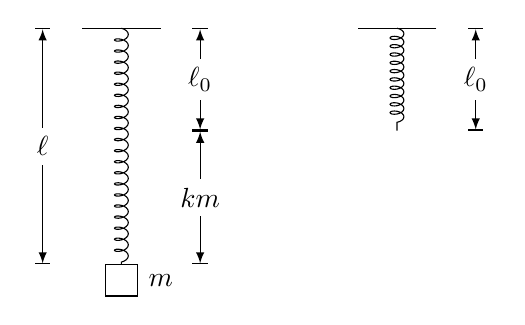
\begin{tikzpicture}[>=latex]
    \draw (-.5,0)--(.5,0);
    \draw (4,0)--(3,0);
    \draw [decorate,decoration={coil,segment length=4pt}](0,0)--(0,-3);
    \draw [decorate,decoration={coil,segment length=3pt}](3.5,0)--(3.5,-1.3);
\draw (-.2,-3) rectangle (.2,-3.4);
\node at (.5,-3.2){$m$};

\draw [|<->|](-1,0)--node[fill=white]{$\ell$}(-1,-3);
\draw [|<->|](1,0)--node[fill=white]{$\ell_0$}(1,-1.3);
\draw [|<->|](1,-1.3)--node[fill=white]{$km$}(1,-3);
\draw [|<->|](4.5,0)--node[fill=white]{$\ell_0$}(4.5,-1.3);

    \end{tikzpicture}
 \caption{}
\end{figure}

\begin{example}
    一种保险丝的直径和它所容许通过的额定电流之
    间的数量关系,可以列成下表:
\begin{center}
\begin{tabular}{cccc}
    \hline
    额定电流(I)  &  保险丝直径(d)  &  额定电流(I) &  保险丝直径(d)\\
(安培)  &  (毫米)  &  (安培)  &  (毫米)  \\
\hline
1.0  &  0.28  &  7.5  &  1.25\\
2.0  &  0.52  &  10.0  &  1.51\\
3.0  &  0.71  &  11.0  &  1.67\\
5.0  &  0.98  &  12.0  &  1.75  \\
6.0  &  1.02  &  15.0  &  1.98\\
\hline
\end{tabular}
\end{center}


\end{example}

\begin{example}
    某地气象站的温度自动记录仪描绘了某一天的温
    度变化曲线,如图4.2.
\end{example}

\begin{figure}[htp]
    \centering
\begin{tikzpicture}[>=latex]
\draw[->](-1,0)--(7.5,0)node[right]{$t$小时};
\draw[->](0,-2.5)--(0,2.5)node[right]{$T^{\circ}{\rm C}$};     
\draw [domain=.1:7, samples=1000, ultra thick] plot(\x, {-1.2*sin(\x r)});

\foreach \x in {-6,-4,...,6}
{
    \draw (0,\x*.3)node[left]{$\x$}--(.1,\x*.3);
}
\foreach \x in {2,4,...,24}
{
    \draw (\x*.28,0)node[below]{$\x$}--(\x*.28,0.1);
}


\end{tikzpicture}
    \caption{}
\end{figure}


我们看到在上面的每个例子中都两个变量;例4.1是弹
簧的长度$\ell$和砝码的重量$m$; 例4.2是额定电流$I$和保险丝直
径$d$; 例4.3是时间$t$和温度$T$. 但是在每个例子中的两个变
量并不是孤立的,它们之间有某种关系,如例4.1中,弹簧秤
长度随砝码的重量$m$的变化而变化;在例4.2中,从表中看
出,保险丝直径$d$的大小要随用电器的额定电流$I$的强度
来选择;在例4.3中,由图纸上的曲线看出,随着时间$t$变化,
温度$T$也随之变化,这三个例子用三种不同的形式(解析式、
表格、图象)描述了两个变量之间的依赖关系.

从上面三个例子中可以看到一个共同点,即一个变量可
在某一范围内“自由变化”,我们把这种变量称为自变量(如
例4.1的砝码重量$m$, 在例4.2的表中所列出的额定电流$I$, 例4.3
的时间$t$), 而另一个变量是随着自变量相应地跟着变动的,
这种变量叫做因变量,或称为自变量的函数(如例4.1的弹簧
长度$\ell$,例4.2的保险丝直径$d$, 例4.3的温度$T$都是相应自变量的
因变量,或相应自变量的函数).

“自变量可在某一范围内自由变化”和“因变量是随着自
变量相应地跟着变动”的意思是,“自变量在某一给定的范围
内可以取每一个值,因变量就按照一定的规律取相应的值”.

在如上所述的各种变化过程中,为了把这种动态的事物
的数量变化关系表达出来,在数学上,我们用“变数符号”去表
达变量;用“函数关系”去表达变量之间的相互关联,函数概
念的明确定义如下:

\begin{blk}{定义 }
    如果有两个变量$x$和$y$, 对于变量$x$在某一给定范
围内的每一确定的值,变量$y$按照一个确定的法则有唯一确
定的值和它对应,那么变量$y$就叫做变量$x$的函数,并把$x$叫做
自变量,$y$也可以叫做因变量,自变量的取值范围叫做这个
函数的定义域,在这个定义域上,因变量$y$的取值范围叫做这
个函数的值域.
\end{blk}


这样,在例4.1中弹簧长度$\ell$是砝码重量$m$的函数,例4.2中保
险丝直径$d$是额定电流$I$的函数,例4.3中温度$T$是时间$t$的函数.

这个函数定义包含着三个要素:定义域、对应
法则、值域.

为了正确地理解函数定义,下面我们进一步来剖析一
下:

\subsubsection{函数的定义域}
所谓函数的定义域,就是自变量容许取值的范围,也就
是自变量所取数值的集合.

为以后表述简单起见,在进一步讲解函数的定义域之
前,先介绍一下区间的概念.

我们把数集$\{x|a<x<b\}$记作$(a,b)$, 称为以$a,b$为端点
的开区间,把数集$\{x|a\le x\le b\}$记作$[a,b]$, 称为以$a,b$为端
点的闭区间,而象$(a,b]$和$[a,b)$都称为半开区间,它们分别
是数集$\{x|a<x\le b\}$和$\{x|a\le x<b\}$, 我们把各种区间记号及
其所表示的点(数)集并列如下:
\begin{multicols}{2}
    \begin{enumerate}
    \item $(a,b)=\{x|a<x<b\}$
    \item $ [a,b]=\{x|a\le x\le b\}$
    \item $(a,b]=\{x|a<x\le b\}$
    \item $[a,b)=\{x|a\le x<b\}$
    \item $(a,+\infty)=\{x|x>a\}$
    \item $[a,+\infty)=\{x|x\ge a\}$
    \item $(-\infty,b)=\{x|x<b\}$
    \item $(-\infty,b]=\{x|x\le b\}$
    \item $(-\infty,+\infty)=\mathbb{R}$ (实数集)
\end{enumerate}
\end{multicols}

其中5--9中有无穷大$+\infty$, $-\infty$, 它们是一种记号而
不是一个数,下列记号不论哪一个都是无意义的:$(a,+\infty]$,
$[a,+\infty]$, $[-\infty,b)$, $[-\infty,b]$或$[-\infty,+\infty]$

以后某些数集就可以用区间来表示.

谈到函数,就要指明定义域,离开定义域去谈函数是没
有意义的,定义在$(-\infty,+\infty)$上的关于$x$的函数$y=x^2$和定
义在$[0,+\infty)$上的关于$x$的函数$y=x^2$, 尽管函数表达式是
一样的,但由于定义域不同,故不能认为这两个函数是一样
的.

怎样确定一个函数的定义域呢?一般有两个途径.
\begin{enumerate}
    \item 在实际问题中函数的定义域根据实际问题的意义来
    定.

    例如,例4.3温度自动记录仪记录下的一昼夜的气温$T$的变
    化情况,这里气温$T$是时间$t$的函数,自变量$t$的容许值范围
    是$[0,24]$.

    \item 在理论上研究函数时,定义域或者已经明确给出,
    或者由函数表达式确定.

    如果我们讨论的函数由一个数学算式表示,并且不考虑
    它的实际意义,那么这个函数的定义域,就是指使这个数学
    算式有意义的自变量取值范围,这又叫做自然定义域,通常
    不需要明确指出.

    例如,函数$\frac{1}{x}$
    的定义域是由除零以外的一切实数所组
    成,即$(-\infty,0)\cup(0,+\infty)$, 又如函数$\sqrt{x}$的定义域是一切
    正数和零所组成,即$[0,+\infty)$.
\end{enumerate}


\begin{example}
 在一个边长为30cm
的正方形铁皮上,四角各截去
边长为$x$的小正方形(图4.3),
按虚线折起来成一个无盖盒
子,求这个盒子容积$V$关于自
变量$x$的函数关系,并指明其
定义域.   
\end{example}

\begin{figure}[htp]
    \centering
\begin{tikzpicture}[>=latex]
\draw (0,0) rectangle (4,4);
\draw[pattern=north east lines] (0,0) rectangle (.75,.75);    
\draw[pattern=north east lines] (3.25,0) rectangle (4,.75);  
\draw[pattern=north east lines] (0,3.25) rectangle (.75,4);  
\draw[pattern=north east lines] (3.25,3.25) rectangle (4,4);  
\draw[dashed] (0.75,0.75) rectangle (3.25,3.25);  
\foreach \x in {0,4}
{
    \draw (\x,4)--(\x,4.8);
}
\draw [<->](0,4.4)--node[fill=white]{30}(4,4.4);
\foreach \x in {0,.75,3.25,4}
{
    \draw (\x,0)--(\x,-.8);
}
\draw [<->](0.75,-.4)--node[fill=white]{$30-2x$}(3.25,-.4);
\draw [<->](0.75,-.4)--node[below]{$x$}(0,-.4);
\draw [<->](4,-.4)--node[below]{$x$}(3.25,-.4);
\end{tikzpicture}
    \caption{}
\end{figure}

\begin{solution}
    已知截去小正方形边
    长为$x$cm, 做成的盒子的高是
    $x$cm,盒子的边长是$(30-2x)$cm.
\[\therefore\quad     V=x(30-2x)^2\]
    这就是所求的$V$关于$x$的函数.

    根据实际问题,小正方形的边长不能为零或负数,另一
    方面它又不能等于或大于正方形边长的一半,所以$x$只能在0
    和15之间,故函数的定义域是$(0,15)$.
\end{solution}

\begin{example}    
    求下列$x$的函数的定义域:
    \begin{multicols}{2}
\begin{enumerate}
    \item $y=x+1$
    \item $y=\frac{x^2+1}{x-1}$
    \item $y=\sqrt{3-x}$
    \item $y=\sqrt{3-x}+\sqrt{x+3}$
    \item $\frac{1}{\sqrt[3]{x+4}}$
    \item $\frac{\sqrt{x+1}}{x^2-5x+6}$
    \item $\lg(1-\sqrt{3-x})$
\end{enumerate}        
    \end{multicols}
\end{example}

\begin{solution} 
\begin{enumerate}
    \item $y=x+1$的定义域为实数集$\mathbb{R}$,即:$(-\infty,+\infty)$.
    \item $y=\frac{x^2+1}{x-1}$的定义域为$x\ne 1$的一切实数,即
    \[x\in (-\infty,1)\cup(1,+\infty)\]
\item $y=\sqrt{3-x}$,要使根式有意义,就要$3-x\ge 0$,
即$x\le 3$, 即$x\in (-\infty,3)$.
\item $y=\sqrt{3-x}+\sqrt{x+3}$要使两个根式同时有意义,定义域只能是每个根式的定
义域的交集.
\begin{itemize}
    \item $3-x\ge 0$的解集是$(-\infty,3)$;
    \item  $x+3\ge 0$的解集是$(-3,+\infty)$.
\end{itemize}
因此,$x\in (-\infty,3)\cap (-3,+\infty)=[-3,3]$ (图4.4)
\begin{figure}[htp]
    \centering
\begin{tikzpicture}[>=latex]
\draw[->] (-4,0)--(4,0)node[right]{$x$};
\foreach \x in {-3,0,3}
{
    \draw (\x,0)node[below]{$\x$}--(\x,.1);
}
\draw (-3,0)--(-3,1)--(4,1);
\draw (3,0)--(3,.5)--(-4,.5);
\draw[pattern=north east lines] (-3,.5) rectangle (3,0);
\end{tikzpicture}
    \caption{}
\end{figure}
\item 要使式子$\frac{1}{\sqrt[3]{x+4}}$有意义,就要$x+4\ne 0$, 即$x\ne -4$,所以定义域是$(-\infty,-4)\cup(-4,+\infty)$.
\item 要使式子$\frac{\sqrt{x+1}}{x^2-5x+6}$有意义,必须且只须,
\[\begin{cases}
    x+1\ge 0\\
x^2-5x+6\ne 0
\end{cases}\Rightarrow\quad \begin{cases}
   x\ge -1\\
   x\ne 2\quad x\ne 3 
\end{cases}\]
故定义域是$[-1,2)\cup(2,3)\cup(3,+\infty)$ (图4.5).

\begin{figure}[htp]
    \centering
    \begin{tikzpicture}[>=latex]
        \draw[->] (-2,0)--(5,0)node[right]{$x$};
\foreach \x in {-1,2,3}
{
    \draw (\x,0)node[below]{$\x$}--(\x,.5);
}

\node at (0,0)[below]{0};

\draw (-1,0.5)--(4.5,.5);
\fill[pattern=north east lines] (-1,.5) rectangle (4.5,0);
\draw(-1,0)[fill=black] circle (1.5pt);
\draw(2,0)[fill=white] circle (1.5pt);
\draw(3,0)[fill=white] circle (1.5pt);
    \end{tikzpicture}
    \caption{}
\end{figure}

\item 要使对数$\lg(1-\sqrt{3-x})$的真数中的根式有意
义,只要
$3-x\ge 0$, 
要使对数有意义,又必须且只须真数大于零,即
$1-\sqrt{3-x}>0$,
因此要使对数$\lg(1-\sqrt{3-x})$有意义,必须且只须使
$x$满足下面不等式组:
\[\begin{cases}
    3-x\ge 0\\
\sqrt{3-x}<1
\end{cases}\Rightarrow\quad \begin{cases}
    x\le 3\\
x>2
\end{cases}\]
所以函数$\lg(1-\sqrt{3-x})$的定义域是$(2,3]$. 

\end{enumerate}    
\end{solution}

\subsubsection{对应法则}
对应法则是因变量$y$对自变量$x$的依赖关系(即函数关
系)的具体表现,它是函数概念里最本质的东西,也是区别
各个不同函数的最主要的标志.定义在$(-\infty,+\infty)$上$y$对$x$的
函数:$y=x^2$, 和定义在$(-\infty,+\infty)$上$U$对$V$的函数:$U=V^2$, 
尽管自变量与因变量各用不同的字母,但由于它们的对应法
则是一样的,定义域又相同,故我们不认为它们是不一样的
函数.

应当指出,自变量$x$在某一范围内的每一个值,通过对
应法则,变量$y$有唯一确定的值与之对应,这种对应法则才
体现了因变量$y$与自变量$x$的函数关系,不然的话,尽管给出
了对应法则,但并不构成函数,例如,$x^2+y^2=1$或$y=
\pm\sqrt{1-x^2}$, 当自变量$x$在$-1$到1之间变动时,根据对应法
则,变量$y$就有确定的两个值与之对应,因之对应法则$y=
\pm\sqrt{1-x^2}$, 就不能表现$y$是$x$的函数.但是我们倒可以把这个
对应法则拆成下面两个函数:
\[y=\sqrt{1-x^2},\qquad y=-\sqrt{1-x^2},\quad x\in [-1,1]\]

对应法则的表现形式是各种各样的.一种是用数学公式
来表示函数关系,叫做\textbf{解析式表示法}(如例4.1);一种是列出
对应的数值表来表示函数关系,叫做\textbf{列表表示法}(如例4.2),
还有一种是用图象来表示,叫做\textbf{图象表示法}(如例4.3), 这三
种表示法各有优缺点,解析表示法具有全面、简明的优点,
但自变量与因变量值的对应情况不能直观地反映出来;列
表法虽具有这方面的优点,但对定义域中每个对应值不能完
全列出,不能完全地把函数全貌表达出来;图象法其优点在
于形式简明直观便于比较,易显出数据中的转折点,最高点
或最低点,缺点是不够精确,不便于运算.这里要指出的
是,在实际问题中,这三种方法常常是综合使用的,例如在
作函数图象时,是由解析式→列表→图象,而在根据实
验数据求出一般公式时,常常是把对应数据列成表格,然
后描绘图象,最后根据图象再去寻找相应的公式.

当我们泛指一般函数关系时,就必须舍弃对应法则的具
体表现形式,而只顾及它们的本性——因变量$y$和自变量$x$
之间的依赖关系,采用记号
\[y=f(x)\]
来表达$y$是$x$的函数.注意,记号中的$f$表示某种对应法则.

为简便起见,我们常常用函数的一般记号$y=f(x)$来代
表一个具体函数.如例4.1, 可以用$\ell=f(m)$来表示,不过这里
的$f(m)$应理解为例4.1的具体的对应法则:$f(m)=km+\ell_0$

关于函数的记号,还应注意:
\begin{enumerate}
    \item 例如,圆面积$A$和周长$C$都是半径$r$的函数,如果我
    们都用
 \[   A=f(r),\qquad C=f(r)\]
    来表示,那么这里的$f(r)$是指$2\pi r$还是$\pi r$呢?就分不清了,
    所以,在同时研究这两个函数时,为避免混淆,就须在括号
    外面选用不同的字母,以区别这两个不同的函数关系,比如
    \[   A=f(r),\qquad C=g(r)\]
    \item 认识一个函数,关键就在于认识“$f$”,自变量与因
    变量用什么宇母表示是无关紧要的.

    如果“$f$”是以解析式给出,那么“$f$”就是这个解析式所
    含的一系列按一定顺序的运算.例如,函数
 \[   f(x)=x^2-3x+5\]
    这里“$f$”是指对自变量$x$实行下述运算后求得对应的函数值:
\[\text{(自变量)}^2-3\x \text{(自变量)}+5\longrightarrow \text{对应的函数值}\]
如$f(2)$就是对“2”实行这套运算,即$2^2-3\x 2+5=3$, 
    得到$f(2)=3$.
\end{enumerate}

\subsubsection{函数值域}
当函数的自变量$x$取遍定义域$D$中的一切值时,所对应
的函数值$y$的全体构成集合$R=\{y|y=f(x),\; x\in D\}$. 我们称
集合$R$是这函数的值域.由值域的定义易知对任意的$y_0\in R$,
必有$x_0\in D$与之对应,使关系式$y_0=f(x_0)$成立,但是与这$y_0$对
应的$x$值可能不止一个,例如$y=|x|$, 与$y=4$对应的$x$值有两
个:$x=4$或$x=-4$.再看一例,$y=f(x)=3$, $x\in D=(-\infty,+\infty)$, $R=\{3\}$, 这函数的值域是单元素集,只由一
个数3组成.这个函数称为常值函数,而与$y=3$对应的$x$值有
无穷多个,即一切实数.

\section*{习题4.1}
\addcontentsline{toc}{subsection}{习题4.1}
\begin{enumerate}
    \item     求下列函数的定义域($y$是$x$的函数):
    \begin{multicols}{2}
\begin{enumerate}
    \item $y=2x^2-3$
    \item $y=\sqrt{x}$
    \item $y=\sqrt{x-5}$
    \item $y=\sqrt{x^2-9}$
    \item $y=\lg(-x^2+9)$
    \item $y=\sqrt{x^2+9}$
    \item $y=\frac{x+1}{x-3}$
    \item $y=\sqrt{x^2-8x+15}$
    \item $y=\frac{\sqrt{x-1}}{x-5}$
    \item $y=\sqrt{x-4}+\sqrt{6-x}$
    \item $y=\sqrt{x^2-5x+4}+\lg(x+2)$

\end{enumerate}        
    \end{multicols}

\item 已知$f(x)=7x(2x-5)$, 求函数$f(x)$在$x=0,\frac{1}{2},1,2,
    \frac{1}{2+\sqrt{3}}$处的值.
    
\item 已知自变量$x$与因变量$y$之间有下面的关系,用$x$的代数
    式来表达$y$, 给出函数的定义域.
\begin{multicols}{2}
\begin{enumerate}
    \item $3x+4y=12$
    \item $xy=15$
    \item $(x-2)(y+3)=-6$
    \item $x=\frac{5y+3}{3y+2}$
\end{enumerate}
\end{multicols}

\item 试将$n$边形对角线的数目$N$用边数$n$的函数写出来,并指
出这函数的定义域.
\item 三角形两边的长$a,b$一定,夹角$\theta$不定,写出三角形面积
对于夹角$\theta$的函数关系,并指出这函数的定义域.
\item 圆的半径$R$一定,如果圆内扇形的中心角$\theta$是个变量,
求扇形面积$A$对于中心角$\theta$的函数,这里半径$R$的单位是
厘米,$\theta$的单位是度,又如果扇形中心角的单位改用弧
度,那么这个函数关系表达式有何改变?
\item 人工开凿的直线运河经过相距$d$公里的$A,B$两城(图
4.6).在$B$城垂直于运河的方向上离$B$城$\ell$公里有一个工
厂$C$, 从$A$城运货到工厂,先从水路到一地$M$, 然后走
陆路从$M$到$C$. 假设一吨货物每公里水路运费为$\alpha$元,陆
路运费为$\beta$元,求每吨总运费与$MB$之间的函数关系.
\begin{figure}[htp]
    \centering
\begin{tikzpicture}[>=latex, scale=.8]
\draw (0,0)node[left]{$A$}--(8,0)node[above]{$B$};
\draw (5,0)node[above]{$M$}--(8,4)node[above]{$C$};    
\draw[dashed](8,4)--(8,0);
\foreach \x in {0,5,8}
{
    \draw (\x,0)--(\x,-.8);
}
\draw[<->] (0,-.6)--node[fill=white]{$d$}(8,-.6);
\draw[<->] (5,-.3)--node[fill=white]{$x$}(8,-.3);
\draw[|<->|] (8.3,0)--node[fill=white]{$\ell$}(8.3,4);

\end{tikzpicture}
    \caption{}
\end{figure}


\item  在底为$AC=b$和高为$BD=h$的三角形$ABC$中(图4.7)内
接一个高为$NM=x$的矩形$KLMN$, 把矩形$KLMN$的周长
$P$及其面积$S$表示为$x$的函数.
\begin{figure}[htp]
    \centering
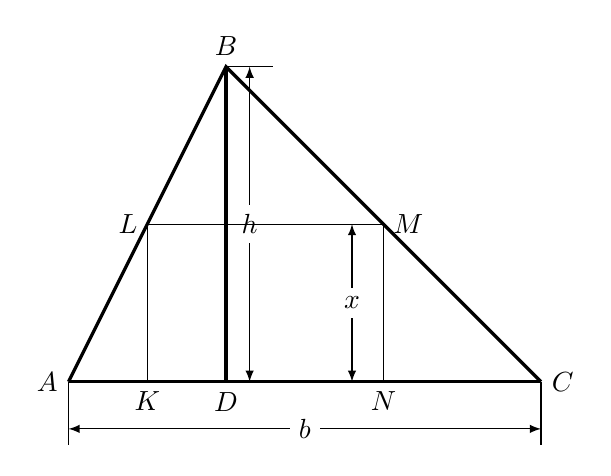
\begin{tikzpicture}[>=latex]
\draw[very thick] (0,0)node[left]{$A$}--(6,0)node[right]{$C$};
\draw[very thick] (0,0)--(2,4)node[above]{$B$}--(6,0);
\draw[very thick] (2,4)--(2,0)node[below]{$D$};  
\draw[<->](2.3,0)--node[fill=white]{$h$}(2.3,4);
\draw (1,0)node[below]{$K$}--(1,2)node[left]{$L$} --(4,2)node[right]{$M$}-- (4,0)node[below]{$N$};
\draw (2,4)--(2.6,4);

\draw[<->](3.6,0)--node[fill=white]{$x$}(3.6,2);
\foreach \x in {0,6}
{
    \draw (\x,0)--(\x,-.8);
}
\draw[<->](0,-.6)--node[fill=white]{$b$}(6,-.6);

\end{tikzpicture}
    \caption{}
\end{figure}

\item 金属切削加工时,刀具一分钟内在零件(工件)表面上所
经过的路程(如铣床),或工件每分钟在刀具上所经过的
路程(车床),叫做切削速度,设:
$D$是刀具或工件直径(毫米);
$n$是刀具或工件每分钟转数;
$v$是切削速度(米/分).
那么切削速度$v$,对于刀具或工件的每分钟转
数$n$的函数关系是:
\[v=\frac{\pi Dn}{1000}\]
你能推导出这个关系式吗?
\item $y=f(x)=\begin{cases}
    \frac{1}{x} & 0<x\le 1\\ 0& x=0
\end{cases}$
是不是定义在$[0,1]$上的函数?为什么?值域是什么?又
$f(x)=\frac{1}{x}$
是不是定义在$[0,1]$上的函数?
\end{enumerate}

\subsection{函数的图象}
我们指出过,几何图形是符合某种条件的点的集合,例
如以$r$为半径的圆$O$是与$O$点距离等于定长$r$的点的集合,线段
的垂直平分线是和$A,B$的距离相等的点的集合.

我们也讲过有序实数对和坐标平面上的点是一一对应
的,即每个有序实数对对应着平面上一个点而且只对应一个
点,反之,平面上的每个点对应着一个有序实数对而且只对
应一个有序实数对.

根据这样的思想,我们来建立函数图象的概念.

已知函数$y=f(x)$, 定义域为$D$.
\begin{figure}[htp]
    \centering
\begin{tikzpicture}[>=latex]
  \draw[->](-.5,0)--(5,0)node[right]{$x$};
    \draw[->] (0,-1)--(0,3.5)node[right]{$y$};
\node at (-.25,-.25){$O$};
\draw (-.5,.5) to [bend right=-14](1,2) to [bend right=-10](4,3)node [right]{$y=f(x)$的图象};
\draw (1,0)node[below]{$x$}--node[right]{$f(x)$}(1,2)node[above]{$(x,f(x))$};
\draw[dashed](1,2)--(0,2)node[left]{$f(x)$};
\end{tikzpicture}
    \caption{}
\end{figure}


对于定义域$D$中任意的$x$, 点$(x,f(x))$表示平面上一个
点.当$x$遍取$D$中的一切值时,点$(x,f(x))$的集合就构 成一个
图形$F$(图4.8). 这个图形$F$就是函数$y=f(x)$的图象.下面给出定义:

\begin{blk}{定义}
函数$y=f(x)$的图象$F$是坐标平面上所有这样的
的图象点的集合:其坐标$(x,y)$由下
列法则给出:
\begin{enumerate}
    \item $x$遍取定义域$D$中
的一切值,
\item $y$由函数关系式$y=f(x)$确定.
\end{enumerate}
用符号表示:
\[F=\{(x,y)|x\in D\; \text{ 且 }\; y=f(x)\}\]    
\end{blk}


由定义知道,要证明图象$F$是函数$y=f(x)$的图象,必
须要证明下面两点:
\begin{enumerate}
    \item  $F$上所有的点的坐标$(x,y)$都能适合$y=f(x)$.
\item 不在$F$上所有的点的坐标$(x,y)$都不适合$y=f(x)$.

(或证2的逆否命题:“坐标能适合$y=f(x)$的关系的点都
在$F$上”也可).
\end{enumerate}

作函数$y=f(x)$的图象就是把$F$上的点都标在坐标平
面上,平面点集$F$一般是个无限集,把$F$的点一个一个地都
标出来是不可能的,在一般情形,我们的办法是先作出图形
$F$的一些点,然后用一条或几条平滑曲线把这些点连接起来
(连结的时候,通常依照自变量由小到大的顺序)而得到图形
$F$.

\begin{example}
描绘函数$y=\frac{1}{2}x^2$的图象.
\end{example}

\begin{solution}
这函数的定义域为一切实数,$x$可取任意实数,如:

取$x=\cdots,\quad -4,\quad -3,\quad -2,\quad -1,\quad 0,\quad 1,\quad 2,\quad 3,\quad 4,\quad \cdots$

计算$y=\cdots,\quad 8,\quad 4.5,\quad 2,\quad 0.5,\quad 0,\quad 0.5,\quad 2,\quad 4.5,\quad 8,\quad \cdots$

得有序对$(x,y)$:$\cdots,\quad (-4,8)$,\quad  $(-3,4.5)$,\quad  $(-2,2)$,\quad  $(-1,0.5)$,\quad  $(0,0)$,\quad  $(1,0.5)$,\quad  $(2,2)$,\quad  $(3,4.5)$,\quad  $(4,8),\quad\cdots$


通常用表格表示:
\begin{center}
\begin{tabular}{c|ccccccccccc}
\hline
$x$ & $\cdots$  &  $-4$  &  $-3$  &  $-2 $ &  $-1$  &  0  &  1  &  2  &  3  &  4  &  $\cdots$\\
\hline
$y$ &$\cdots$  &  8  &  4.5  &  2  &  0.5  &  0  &  0.5  &  2  &  4.5  &  8  &  $\cdots$\\
\hline
\end{tabular}
\end{center}

由这些有序对可在平面上描出对应的点,用平滑曲线把
这些点连接起来,就得到函数$y=\frac{1}{2}x^2$
的图象(图4.9), 这种
描点作图象的方法叫做\textbf{描点法}.
\begin{figure}[htp]
    \centering
\begin{tikzpicture}[>=latex, scale=.7]
    \draw[->](-5,0)--(5,0)node[right]{$x$};
      \draw[->] (0,-1)--(0,9.5)node[right]{$y$};
  \node at (-.35,-.35){$O$};

\foreach \x in {1,2,3,4}
{
    \draw (\x,0)--(\x,.1);
    \draw (-\x,0)--(-\x,.1);
    \draw (0,\x)--(-.1,\x);
    \draw (0,\x+4)--(-.1,\x+4);
}

\foreach \x in {2,4}
{
    \node at (\x,0)[below]{$\x$};
    \node at (-\x,0)[below]{$-\x$};
}

\foreach \x in {2,4,6,8}
{
    \node at (-.1,\x)[left]{$\x$};
}

\draw [domain=-4.2:4.2, samples=100, very thick] plot(\x,{0.5*\x*\x});

\foreach \y in {-4,-3,...,4}
{
    \draw (\y, {0.5*\y*\y})[fill=black] circle (2pt);
}

\node at (5,6){$y=\frac{1}{2}x^2$};
\end{tikzpicture}
    \caption{}
\end{figure}
\end{solution}

应当指出,用描点法作图
象时,我们至多只能描出图象
的有限多个点,而不可能描出
$F$的全部的点,所以这种方法
带有一定盲目性,因为仅有一
些点并不足以确切掌握函数图象全貌,因此我们必须先对这
函数表达式进行详尽的研究,把握这函数图象的某些特点,
如间断点,最高点,最低点,函数变化趋向等,而后根据研
究的结果,结合使用描点法来给出这函数的图象.这是今后要
结合着各种函数逐步深入研究的一个问题.

\begin{ex}
描绘下列函数的图象:
\begin{multicols}{2}
\begin{enumerate}
    \item $y=\frac{1}{2}x^3$
    \item $y=\frac{1}{2}x$
    \item $y=2x+1$
    \item $y=x^2$
    \item $y=\sqrt{x}$
\end{enumerate}
\end{multicols}
\end{ex}

\subsection{正比例函数及其图象}
如果两个变量$x$和$y$之间的相依关系是:当变量$x$依某一
比值变化时,变量$y$按相同比值变化,我们说变量$y$和变量
$x$成正比例变化,或者说变量$y$是变量$x$的\textbf{正比例函数}.

\begin{example}
    我国发射的第一颗人造地球卫星,绕地球一圈平
均运行速度为每秒7.12公里,那么这颗人造地球卫星在2秒钟
内运行了14.24公里,在6秒钟内运行了$7.12\x6=42.72$公
里.如果以公里为单位的路程用$S$表示,以秒为单位的时间
用$t$表示,那么$S$和$t$之间成立下面的等式:
\[S=7.12t\]

容易说明变量$S$和$t$成正比例变化,设$t_1$和$t_2$是时间$t$的任
意两个不等于0的数值,$S_1$和$S_2$是它们的对应值,于是$S_1=
7.12t_1$, $S_2=7.12t_2$, 从而$\frac{S_2}{S_1}=\frac{t_2}{t_1}$
,因此路程$S$是时间$t$的正比例函数.
\end{example}

\begin{example}
    物理学中的虎克定律是“在弹性限度内,弹力跟弹
簧的伸长(或缩短)成正比例”,设弹簧的原长为$\ell_0$(cm), 弹簧
变形后的弹簧长为$\ell$(cm), 当弹簧伸长$\Delta \ell_1=\ell_1-\ell_0$(cm)时,对
应的弹力为$F_1$(kg); 当弹簧伸长$\Delta \ell_2=\ell_2-\ell_0$(cm)时,对应弹
力为$F_2$(kg), 依虎克定律有:
\[\frac{F_2}{F_1}=\frac{\Delta \ell_2}{\Delta \ell_1}\]
也就是:$\frac{F_2}{\Delta \ell_2}=\frac{F_1}{\Delta \ell_1}=k$,这里$k$是常数,在数值上等于弹簧
伸长1cm时对应的弹力数值.因此,弹力$F$与伸长$\Delta \ell$有下面的
关系:
\[F=k\Delta \ell\]
\end{example}

\begin{figure}[htp]
    \centering
\begin{tikzpicture}[>=latex, scale=1.3]
\fill[pattern=north east lines](-1,.25) rectangle  (1,0);
\draw(-1,0)--(1,0);    
\draw [decorate,decoration={zigzag,segment length=8pt}] (0,0)--(0,-1.5);
\draw[dashed](0,-2) circle (.2);
\draw(0,-1.5)--(0,-3);
\draw[dashed](0,-3)--(0,-4);
\draw(0,-3) circle (.2);
\draw[dashed](0,-4) circle (.2);
\draw[dashdotted] (-1,-3)node[left]{$O$}--(1,-3);
\draw (0,-2)--(1,-2);
\draw (0,-4)--(1,-4);
\node at (-.3,-2.75){$m$};
\draw[<->] (-.7,0)--node[fill=white]{$\ell_0$}(-.7,-3);
\draw[<->] (.5,-2)--node[fill=white]{$\Delta \ell$}(.5,-3);
\draw[<->] (.7,-4)--node[fill=white]{$\Delta \ell$}(.7,-3);
\end{tikzpicture}
    \caption{}
\end{figure}
\begin{example}
    让我们考察在弹簧下挂一质量为$m$的小球,如
图4.10, 把小球用力向下拉一段距离后,放开小球就开始振
动.
\begin{itemize}
    \item 如果$\Delta \ell=\ell-\ell_0>0$, $\Delta \ell$是弹
簧伸长量.
\item 如果$\Delta \ell=\ell-\ell_0<0$, $\Delta \ell$是弹
簧压缩量.
\end{itemize}

因为要拉长或压缩弹簧,必
须要有跟拉长或压缩的大小成正
比例(在某一限度内)的力,因此
当小球移到离开平衡位置 $\Delta \ell$的距
离处,这时小球所受恢复力$F$就是:
\[F=-k \Delta \ell\]

式中$k$是弹簧的弹性系数,它在数值上等于弹簧伸长
或压缩单位长度时所产生的弹力.在上式中我们还把在一条
有向直线上的位移的方向和弹力的方向考虑进来,上面等式
中的负号表示力和位移的方向相反.
\end{example}

从上面几个例子得知,正比例函数的一般解析式是:
\[y=kx,\quad  k\ne 0,\quad  x\in(-\infty,+\infty)\]

在函数研究中常用上面的解析式作为正比例函数的定
义.

\begin{blk}{定义}
    函数$y=kx$($k$是不等于零的常数)叫做正比例函
数,这里常数$k$叫做变量$y$对变量的比例系数,它的数值等于自
变量取数值1时,因变量$y$的对应值.
\end{blk}

下面我们来证明正比例函数$y=kx\; (k\ne 0)$的图象是一条
过原点和点$N(1,k)$的直线.

为简单起见,设$k>0$,根据函数图象的定义,要证直线$ON$是$y=kx$的图象,就要证明下面两个命题:
\begin{enumerate}
    \item 在直线$ON$上的每一个点的坐标都满足$y=kx$;
    \item 不在直线$ON$上的任何一点,它的坐标$(x,y)$都不
满足$y=kx$.
\end{enumerate}

我们来证1:
\begin{itemize}
    \item 令$x=0$, 则$y=k\cdot 0=0$,即原点$(0,0)$在函数$y=kx$
的图象上.
\item 令$x=1$,则$y=k\cdot 1=k$,即点$N(1,k)$在$y=kx$的图象上.
\end{itemize}

过原点和$N(1,k)$点作一
条直线(图4.11),现在需要证
明直线$ON$上的每一个点的坐标都满足$y=kx$.

\begin{figure}[htp]
    \centering
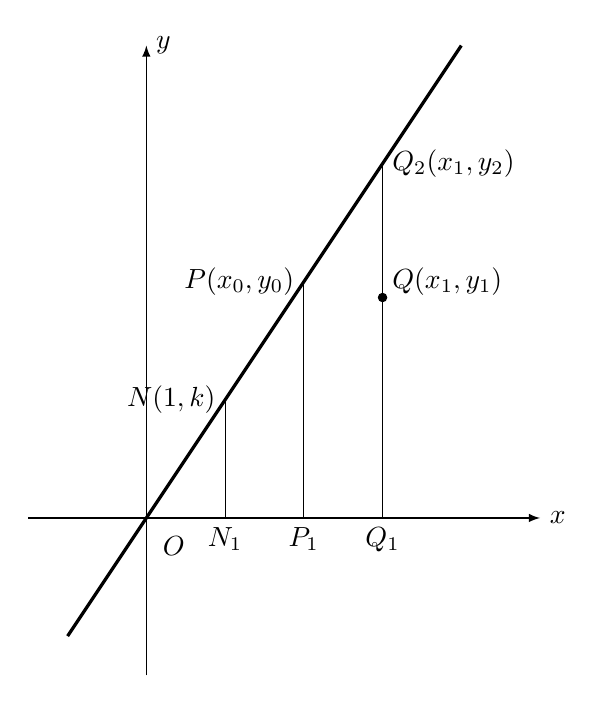
\begin{tikzpicture}[>=latex]
    \draw[->](-1.5,0)--(5,0)node[right]{$x$};
    \draw[->] (0,-2)--(0,6)node[right]{$y$};
\node at (.35,-.35){$O$};
\draw[very thick] (-1,-1.5)--(4,6);    
\draw (1,0)node[below]{$N_1$}--(1,1.5)node[left]{$N(1,k)$};
\draw (2,0)node[below]{$P_1$}--(2,3)node[left]{$P(x_0,y_0)$};
\draw (3,0)node[below]{$Q_1$}--(3,4.5)node[right]{$Q_2(x_1,y_2)$};
\node at (3,3)[right]{$Q(x_1,y_1)$};
\draw (3,2.8)[fill=black] circle (1.5pt);
\end{tikzpicture}
    \caption{}
\end{figure}

在直线$ON$上任取一个不同于$O,N$的点$P(x_0,y_0)$, 过$N,P$
两点作直线$N_1N$和$P_1P$平行于$y$轴且和$x$轴分别交于$N_1(1,0)$
和$P_1(x_0,0)$二点,

$\because\quad N_1N\parallel P_1P\qquad \therefore\quad \triangle ON_1N\sim \triangle OP_1P$,故有
\[\frac{|P_1P|}{|OP_1|}=\frac{|N_1N|}{|ON_1|}\]
而$ON_1=1$, $N_1N=k$, 因此
\[\frac{|P_1P|}{|N_1N|}=k\]
又因为$P_1P$, $N_1N$分别是$P$点的纵坐标和横坐标且同号,从而有:
\[\frac{y_0}{x_0}=k\quad \Rightarrow\quad y_0=kx\]
这就证明了$(x_0,y_0)$满足关系$y=kx$.

再来证2:设$Q(x_1,y_1)$点不在直线$ON$上,过$Q$点作直线平行于$y$轴,
交直线$ON$于$Q_2(x_1,y_2)$点,交$x$轴于$Q_1(x_1,0)$点,则$OQ_1=
x_1$. 因为$Q_2$点在直线$ON$上,据1的证明,它的坐标满足$y=
kx$, 即有:
\[\frac{Q_1Q_2}{OQ_1}=\frac{y_2}{x_1}=k\]
另一方面,$Q$点不在直线$ON$上,故$y_2\ne y_1$, 因而
\[\frac{y_1}{x_1}\ne \frac{y_2}{x_1}=k\]
所以 $y_1\ne kx_1$. 这就是说$(x_1,y_1)$不满足$y=kx$.

综合1、2我们得到结论:函数$y=kx$的图象 是过
$O(0,0)$, $N(1,k)$的一条直线.

在$k<0$的情形,用同样的证法得到同样的结论.

函数$y=kx$的图象,以后简称为直线$y=kx$.

现在我们来研究,在比例系数$k$变化的时候,直线$y=kx$
的位置怎样变化.

在画图象时,我们应用上面的结论:正比函数$y=kx$的
图象是通过原点和$N(1,k)$的直线.

对于同一个坐标平面,作函数$y=\frac{1}{2}x$,
$y=x$, $y=2x$
的图象(图4.12),这里三个比例系数都是正的,并且是依
次增加的,从图里可以看出,按照比例系数的增加,函数的图
象渐渐离开$x$轴而接近$y$轴.

对于同一·坐标平面,作函数$y=-\frac{1}{4}x$, $y=-x$, $y=
-3x$的图象(图4.13).这里三个比例系数都是负的,并且
它们的绝对值也是依次增加的.从图里可以看出,按照比例
系数的绝对值增加,函数的图象也渐渐离开$x$轴而接近于$y$轴.
\begin{figure}[htp]\centering
\begin{minipage}[t]{0.48\textwidth}
\centering
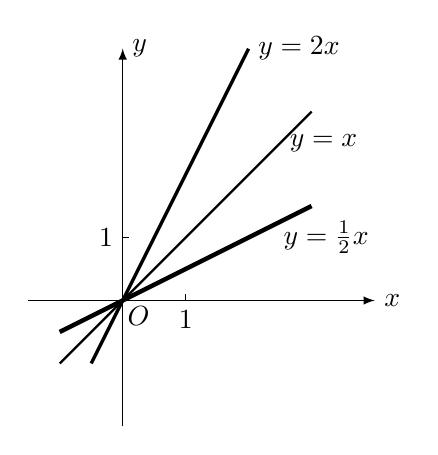
\begin{tikzpicture}[>=latex, scale=.8]
    \draw[->](-1.5,0)--(4,0)node[right]{$x$};
    \draw[->] (0,-2)--(0,4)node[right]{$y$};
\draw [thick, domain=-1:3, samples=100] plot(\x, {\x});
\draw [very thick, domain=-.5:2, samples=100] plot(\x, {2*\x});
\draw [ultra thick, domain=-1:3, samples=100] plot(\x, {0.5*\x});
\draw (1,0)node[below]{1}--(1,.1);
\draw (0,1)node[left]{1}--(.1,1);
\node at (2,4) [right]{$y=2x$};
\node at (2.5,2.5) [right]{$y=x$};
\node at (2.4,1) [right]{$y=\frac{1}{2}x$};
\node at (.25,-.25){$O$};
\end{tikzpicture}
\caption{}
\end{minipage}
\begin{minipage}[t]{0.48\textwidth}
\centering
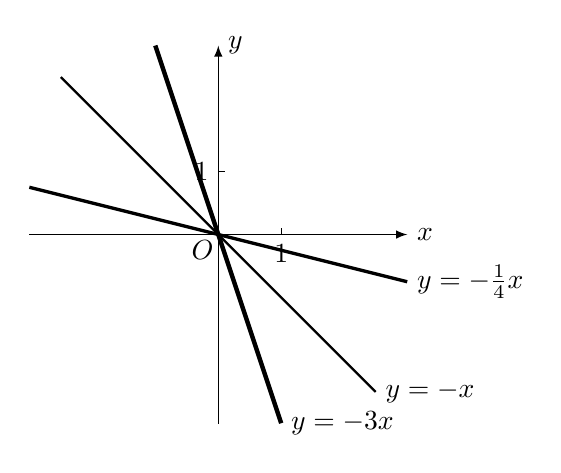
\begin{tikzpicture}[>=latex, scale=.8]
    \draw[->](-3,0)--(3,0)node[right]{$x$};
    \draw[->] (0,-3)--(0,3)node[right]{$y$};
    \node at (-.25,-.25){$O$};
    \draw (1,0)node[below]{1}--(1,.1);
    \draw (0,1)node[left]{1}--(.1,1);
    \draw [thick, domain=-2.5:2.5, samples=100] plot(\x, {-\x});
    \draw [very thick, domain=-3:3, samples=100] plot(\x, {-0.25*\x});
    \draw [ultra thick, domain=-1:1, samples=100] plot(\x, {-3*\x});
    \node at (3,-.75) [right]{$y=-\frac{1}{4}x$};
    \node at (2.5,-2.5) [right]{$y=-x$};
    \node at (1,-3) [right]{$y=-3x$};
\end{tikzpicture}
\caption{}
\end{minipage}
\end{figure}


因此,比例系数$k$和直线$y=kx$与$x$轴正方向所成的角有
关,$k$叫做直线$y=kx$的\textbf{斜率}.

不难证明$k=\tan\alpha,\; 0\le \alpha<180^{\circ},\; \alpha\ne 90^{\circ}$. 这里$\alpha$是直线
向上方向和$x$轴正方向所成的角.

事实上,当$k>0$时,图象为过$O(0,0)$, $N(1,k)$二点,在
一、三象限的直线(图4.14), 那么显见$\tan\alpha=\frac{k}{1}=k$.

当$k<0$时,图象为过$O(0,0)$, $N(1,k)$二点,在二、四象
限的直线(图4.15),这时直线向上方向与$x$轴正的方向所成
的角$\alpha$为钝角.设$\alpha$的补角为$\alpha'$, $k$的相反数$k'=-k>0$, 由
图可见,由于$\triangle ONN_1\simeq \triangle ON'N_1$, $\angle N_1ON'=\angle N_1ON=\alpha'$, $\tan\alpha'=\frac{k'}{1}=k'$, 但
$$\tan\alpha =\tan(180^{\circ}-\alpha')=
-\tan\alpha'=-k'=-(-k)=k$$
 所以$k=\tan\alpha$.

这就是说直线$y=kx$的向上方向与$x$轴正方向所成的角$\alpha$
无论是锐角还是钝角,$\tan\alpha$永远等于比例系数$k$.

\begin{figure}[htp]\centering
\begin{minipage}[t]{0.48\textwidth}
\centering
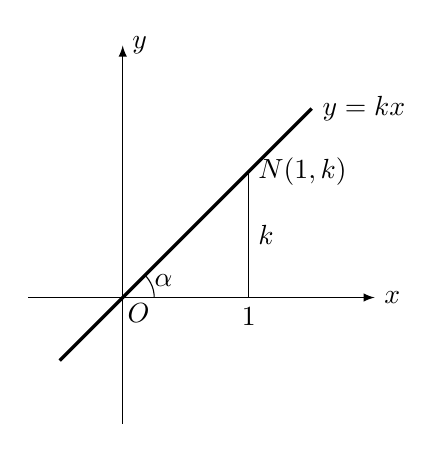
\begin{tikzpicture}[>=latex, scale=.8]
    \draw[->](-1.5,0)--(4,0)node[right]{$x$};
    \draw[->] (0,-2)--(0,4)node[right]{$y$};
\draw[very thick] (-1,-1)--(3,3)node[right]{$y=kx$};
\draw (2,0)node[below]{1}--(2,.1);
\draw (2,0)--node[right]{$k$}(2,2)node[right]{$N(1,k)$};
\node at (.25,-.25){$O$};
\draw (.5,0) arc (0:45:.5); 
\node at (22.5:.7){$\alpha$};
\end{tikzpicture}
\caption{}
\end{minipage}
\begin{minipage}[t]{0.48\textwidth}
\centering
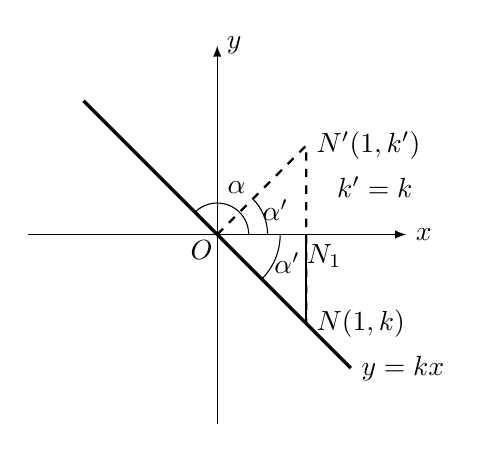
\begin{tikzpicture}[>=latex, scale=.8]
    \draw[->](-3,0)--(3,0)node[right]{$x$};
    \draw[->] (0,-3)--(0,3)node[right]{$y$};
    \node at (-.25,-.25){$O$};
    \draw[very thick] (0,0)--(-45:3)node[right]{$y=kx$};
    \draw[very thick] (0,0)--(135:3);
\draw [dashed, thick](0,0)--(45:2)node[right]{$N'(1,k')$}--(-45:2);
\draw[thick](1.414,0)--(1.414,-1.414)node[right]{$N(1,k)$};
\node at (1.7,0) [below]{$N_1$};
\node at (2.5,.75){$k'=k$};
\draw (.5,0) arc (0:135:.5);
\draw (.8,0) arc (0:45:.8);
\draw (1,0) arc (0:-45:1);

\node at (22.5:1){$\alpha'$};
\node at (-22.5:1.2){$\alpha'$};
\node at (67.5:.8){$\alpha$};

\end{tikzpicture}
\caption{}
\end{minipage}
\end{figure}

如果函数的值随着自变量的值增加而增加,用算式表示
就是:当$x_1<x_2$时,有不等式$f(x_1)<f(x_2)$, 那么函数$f(x)$称为\textbf{递增函数}.

如果函数的值随着自变量的值增加而减少,即当$x_1<x_2$
时,有$f(x_1)>f(x_2)$, 那么函数$f(x)$称为\textbf{递减函数}.

从函数$y=kx$图象可以看出,当$k>0$时,$y=kx$是递增
函数,当$k<0$时,$y=kx$是递减函数.

\section*{习题4.2}
\addcontentsline{toc}{subsection}{习题4.2}
\begin{enumerate}
    \item   下面两个变量是否成正比例变化,试说明之.
\begin{enumerate}
\item 矩形的一条边长固定,它的面积和另一边的长,比
    例系数得什么值.
    \item 圆周上的弧和它所对圆心角.
    \item 正方形的面积和它的边长.
    \item 定圆内的弦长和这弦所对的弧的度数.
    \item $\log_a N$和$\log_b N$, 这里$N>0$.
\end{enumerate}

    \item 圆周长由公式$C=2\pi R$表示,其中$\pi$是无理常数,$R$是
    圆周半径,圆周长与该圆半径成正比例吗?比例系数等
    于什么?怎样用直径表示圆周长?这情形中比例系数得
    什么值?
    \item 水银注入试管时,管底所受压强$p$与注入水银的深度$h$
    成正比,当5厘米深时一平方厘米所受压力等于68克,
    用公式表示$p$因$n$而变的关系.这种情形中的比例系数
    有什么意义?
    \item 
    假如重量不大于100克,也不小于1克,把它悬在钢丝弹
    簧上,弹簧拉长的距离与所悬重量成正比例,当悬挂20
    (g)重物时,弹簧伸长6(mm)
\begin{enumerate}
    \item 用公式表示重量$p$(g)与弹簧加长量$\ell$(cm)间的关系;
    \item 所得公式可以用于
    怎样大的重量.
\end{enumerate}    

    \item 一物体从静止自由落下,从起点所走距离与经过时间的
    平方成正比.如果物体从开始在30秒内落下4410米,在
    一分钟内落下多少米?如果它的速度和经过的时间成正
    比,在2秒末的速度是每秒19.6米,求在10秒末的速
度:
\item \begin{enumerate}
    \item 在同一个坐标系内作下面函数的图象.
    \[y=\frac{1}{3}x,\qquad     y=x,\qquad y=2\frac{1}{2}x,\qquad     y=-3x\]
    \item 求上面各直线的向上方向与$x$轴正方向所成角的大小.
\end{enumerate} 


\item 把汽油用均匀的速度注入桶里,注入的时间和注入的油
量如下:
\begin{center}
\begin{tabular}{c|cccccccc}
    \hline
    注入的时间$t$(分)&1&2&3&4&5&6&7&8\\
   \hline
注入的油量$q$(升)   &2&4&6&8&10&12&14&16\\
   \hline
\end{tabular}
\end{center}
\begin{enumerate}
    \item 找出$t$的任意两个值的比等于$a$的对应的两个值的
    比;
    \item 找出$q$的任意一个值和对应的$t$的值的比;
    \item 用公式表示$q$和$t$间的函数关系;
    \item $q$和$t$是什么关系?
    \item 作出$q$和$t$间的函数关系的图象.
\end{enumerate}
\end{enumerate}


\subsection{反比例函数及其图象}
如果变量$y$和变量$x$的倒数成正比例变化,那么变量$y$叫
做变量$x$的\textbf{反比例函数}.


\begin{example}
    一个物体作匀速运动,行程120米,则运动速度$v$
(米/秒)与所需时间$t$(秒)之间有关系:
\[v=\frac{120}{t}\]
由这关系推知$v$和$t$成反比例变化,事实上,设$t_1$, $t_2$是变量$t$
的任意两个不等于零的数值,$v_1$和$v_2$分别是它们的对应值,于是
\[\frac{v_2}{v_1}=\frac{\frac{120}{t_2}}{\frac{120}{t_1}}=\frac{\frac{1}{t_2}}{\frac{1}{t_1}}\quad \Rightarrow\quad \frac{v_2}{v_1}=\frac{t_1}{t_2}\]
这就是说,变量$v$和变量$t$的倒数成正比例,因此$v$是$t$的反比例
函数,它的解析式是:
\[v=\frac{120}{t}\qquad (t\ne 0)\]
由上式得到$vt=120$, 或$v_2t_2=v_1t_1=$常数,这也就是说,如
果两个变量成反比例变化,那么这两个变量对应值的乘积恒
等于常数,反过来也对.
\end{example}


\begin{example}
    波义耳定律:当温度不变时,一定质量气体的压
强与它的体积成反比.

令体积$V_1$时的压强是$P_1$, 体积$V_2$时的压强是$P_2$. 波义耳
定律的公式表示是:
\[\frac{P_2}{P_1}=\frac{V_1}{V_2}\]
由此得
\[P_1V_1=P_2V_2,\qquad \text{或}\qquad PV=\text{常量}k\]
从而得
\[P=\frac{k}{V}\qquad (V\ne 0)\]

从上面的例子,我们知道反比例函数的一般解析式是:
\[y=\frac{k}{x},\qquad (x\ne 0,\quad k\ne 0)\]

在函数研究中,常用上面的解析式作为反比例函数的定
义.
\end{example}

\begin{blk}{定义}
函数$y=\frac{k}{x}\; (x\ne 0)$叫做反比例函数,这里$k$是
不等于零的常数.
\end{blk}

下面我们来研究函数$y=\frac{k}{x}$的图象.
先来讨论$k$是正数的情形,例如$k=6$.

任意取自变量$x$的一些值(除零以外),算出$y$的对应值,
列表如下:
\begin{center}
\begin{tabular}{c|cccccccccccccccc}
\hline
$x$ & $-8$   &    $-7$   &    $-6$   &    $-5$   &    $-4$   &    $-3$   &    $-2$   &    $-1$   &    $1$   &    $2$   &    $3$   &    $4$   &    $5$   &    $6$   &    $7$   &    $8$\\
\hline
$y$ &$-\frac{3}{4}$&$-\frac{6}{7}$&$-1$&$-1\frac{1}{5}$&$-1\frac{1}{2}$&$-2$&$-3$&$-6$&6&3&2&$1\frac{1}{2}$&$1\frac{1}{5}$&1&$\frac{6}{7}$&$\frac{3}{4}$\\
\hline
\end{tabular}
\end{center}

\begin{figure}[htp]
    \centering
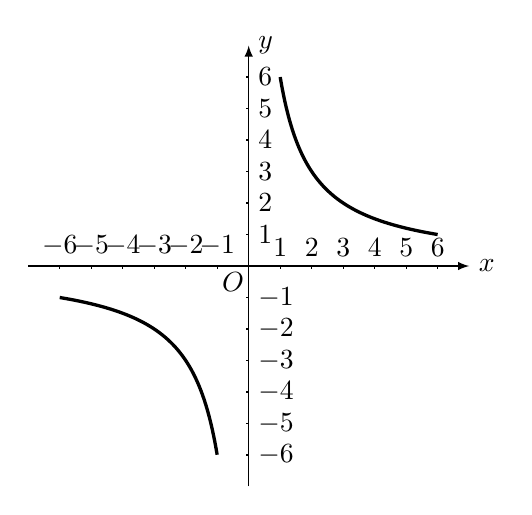
\begin{tikzpicture}[>=latex,scale=.4]
\draw[->] (-7,0)--(7,0)node[right]{$x$};
\draw[->] (0,-7)--(0,7)node[right]{$y$};
\foreach \x in {-6,-5,...,-1,1,2,...,6}
{
    \draw (\x,0)node[above]{$\x$}--(\x,-.1);
    \draw (0,\x)node[right]{$\x$}--(-.1,\x);
}
\draw [domain=-6:-1, samples=100, very thick] plot(\x, {6/\x});
\draw [domain=1:6, samples=100, very thick] plot(\x, {6/\x});
\node at (-.5,-.5){$O$};

\end{tikzpicture}
    \caption{}
\end{figure}

用表里各组对应值作为点
的坐标,在坐标平面上标出各
个点(图4.16).很明显,横坐标
是正的点都在第一象限,横坐
标是负的点都在第三象限(因
为纵坐标与横坐标符号相同),
并且图象与$x$轴和$y$轴都不相交
(因为不可以取$x=0$, 并且不
论取$x$等于什么值,$y$的值都不
会是0).



顺次连结第一象限里的各个点,得到图象的一个分支,
顺次连结第三象限里的各个点,得到图象的另一个分支,这
两个分支合起来就是函数$y=\frac{6}{x}$
图象.

现在我们再来研究$y=\frac{6}{x}$
的图象的一些特点.

当$x$的绝对值逐渐扩大的时候,$y$的绝对值逐渐缩小,但
是不论取$x$等于什么值,$y$的值都不能是零,因此,$y=\frac{6}{x}$的
图象向右和向左都逐渐接近于$x$轴,但是无论什么时候也不
能达到$x$轴.

同样当$x$的绝对值逐渐缩小的时候,$y$的绝对值逐渐扩大,
但是$x$的值不能是零.因此$y=\frac{6}{x}$
的图象向上和向下都逐渐
接近于$y$轴,但是无论什么时候也不能达到$y$轴.

如果$k$是负数,函数$y=\frac{k}{x}$
的图象也有同样的特点,不过
这时图象一个分支在第二象限,另一个分支在第四象限(图
4.17).

$y=\frac{k}{x}$的图象叫做双曲线.

我们也容易看出:如果$k>0$, 它在区间$(-\infty,0)$或$(0,
+\infty)$上是递减函数;如果$k<0$, 它在区间$(-\infty,0)$或$(0,
+\infty)$上是递增函数.

\begin{figure}[htp]
    \centering
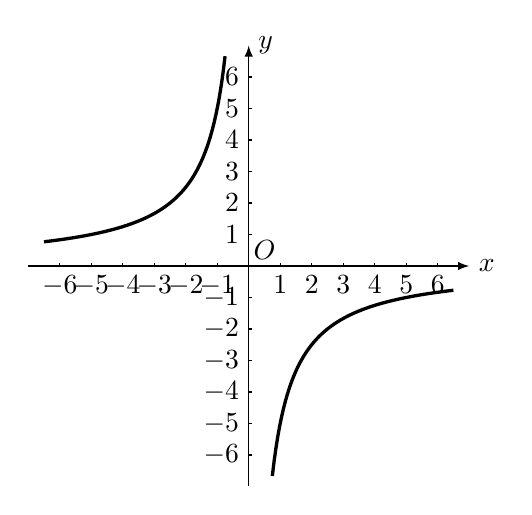
\begin{tikzpicture}[>=latex,scale=.4]
\draw[->] (-7,0)--(7,0)node[right]{$x$};
\draw[->] (0,-7)--(0,7)node[right]{$y$};
\foreach \x in {-6,-5,...,-1,1,2,...,6}
{
    \draw (\x,0)node[below]{$\x$}--(\x,.1);
    \draw (0,\x)node[left]{$\x$}--(.1,\x);
}
\draw [domain=-6.5:-.75, samples=100, very thick] plot(\x, {-5/\x});
\draw [domain=.75:6.5, samples=100, very thick] plot(\x, {-5/\x});
\node at (.5,.5){$O$};

\end{tikzpicture}
    \caption{}
\end{figure}

\begin{ex}
\begin{enumerate}
    \item 下列各种关系里,哪些是正比例关系?哪些是反比例关
    系,哪些都不是,为什么?
    \begin{enumerate}
    \item 完成一定工作的时间和人数(假定每人的工作能力
    相同).
    \item 面积一定的时候,菱形的两条对角线的长.
    \item 被除数相同的时候,除数和商.
    \item 在机车牵引力不变时,消耗的功率与速度.
    \item 在速度维持不变时,消耗的功率与机车牵引力.
    \item 当机车的功率到达定额时,牵引力与速度.
    \item 重量一定的时候,物体的比重和体积.
    \item 体积一定的时候,物体的重量和比重.
    \item 定圆内的弦长和弦到圆心的距离.
    \item 度量一段距离,单位长度与量数.        
    \end{enumerate}

    \item 对于同一个坐标平面,作下列各函数的图象:
    \[y=\frac{8}{x},\qquad y=\frac{4}{x},\qquad y=\frac{2}{x}\]
    \item  对于同一个坐标平面,作下列各函数的图象:
    \[y=\frac{5}{x},\qquad y=-\frac{5}{x}\]
    \item 一工作需要$x-1$个人,用$x+1$天完成,另一工作需要
    $x+2$个人,用$x-1$天完成,且知前一个工作量与后一
    个工作量的比是$9:10$, 求$x$.
\item 从装满纯酒的桶中倒出9升酒后,用水把桶灌满,然后
又倒出9升混合溶液,再用水把桶灌满,这时桶内酒的
体积和水的体积的比是$16:9$, 问桶的容量是多少?
\end{enumerate}
\end{ex}

\section{一次函数(线性函数)}
\subsection{一次函数及其图象}
一次函数的实际例子很多,例如:


\begin{example}
一根长10厘米的弹簧,挂的重量每增加1公斤,
就拉长$\frac{1}{2}$
厘米,那么在弹性限度内,弹簧长度$y$(厘米)与挂
的重量$x$(公斤)之间的函数关系就是:
\begin{equation}
    y=\frac{1}{2}x+10
\end{equation}
\end{example}


\begin{example}
    从北京到广州的包裹邮费为每公斤0.9元,每件另
加手续费0.2元,那么总邮费$y$(元)与包裹重量$x$(公斤)之间
的函数关系就是:
\begin{equation}
  y=0.9x+0.2  
\end{equation}
\end{example}


\begin{example}
    匀速运动中物体离一个定点$O$的距离$S$是用公式:
\[S=vt+S_0\]
表示的,这里$S_0$是物体开始运动的时候离开定点$O$的距离,
$v$是物体运动的速度,它们都是常量,$t$是物体运动的时间,它是自变量,$S$是$t$的一次函数(图4.18).
\begin{figure}[htp]
    \begin{center}
    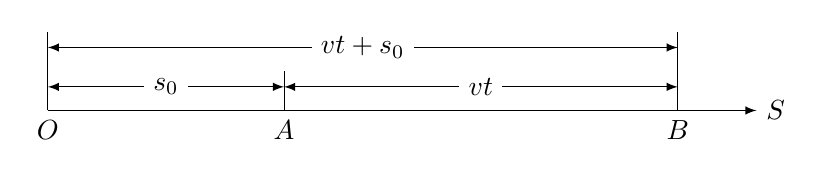
\begin{tikzpicture}[>=latex]
    \draw[->] (0,0)--(9,0)node[right]{$S$};
    \draw (0,0)node[below]{$O$}--(0,1);
    \draw (3,0)node[below]{$A$}--(3,.5);
    \draw (8,0)node[below]{$B$}--(8,1);
    \draw [<->] (0,.3)--node[fill=white]{$s_0$}(3,.3);
    \draw [<->] (8,.3)--node[fill=white]{$vt$}(3,.3);
    \draw [<->] (0,.8)--node[fill=white]{$vt+s_0$}(8,.8);
    \end{tikzpicture}
    \end{center}
    \caption{}
\end{figure}
\end{example}

这三个例子的函数形式都是:
\[y=kx+b\]
其中,$k,b$是两个常量,$k\ne 0$, 这种形式的函数称为\textbf{一次
函数}(或线性函数).其定义域是$(-\infty,+\infty)$, 值域也是
$(-\infty,+\infty)$.

如果$b=0$, 那么$y=kx+b$就成为$y=kx$, 所以正比例
函数是一次函数的特例.

下面讲一次函数的图象是一条直线.

因为正比例函数是一次函数的特例,所以我们可以通过
正比例函数的图象来认识一次函数的图象,并由此认识一般
的图象的平移原理.

为简单起见,假设$b>0$, 从解析式$y=kx+b$和$y=kx$明显
地看出,对于自变量的相同值,一次函数的对应值$y=kx+b$,
总可以由正比例函数$y=kx$的对应值加上$b$得到,这表示
$y=kx+b$的图象上的一切点比直线$y=kx$上具有相同横坐标
的点高出$b$个单位,因此,$x=kx+b$的图象可以由直线沿着$y$
轴向上平移$b$个单位得到,为此在$y$轴上截取线段$OA=b$, 过
$A$点作直线$\ell'$平行于直线$\ell:\; y=kx$ (图4.19).

\begin{figure}[htp]
    \centering
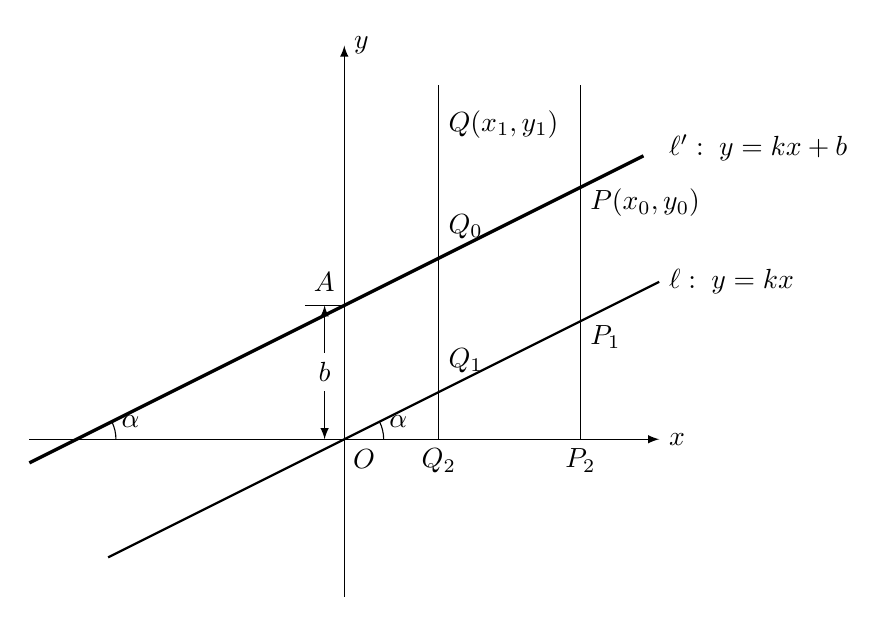
\begin{tikzpicture}[>=latex]
\draw[->] (-4,0)--(4,0)node[right]{$x$};
\draw[->] (0,-2)--(0,5)node[right]{$y$};
\node at (.25,-.25){$O$};

\draw [domain =-3:4, samples=10, thick]plot(\x,{.5*\x});
\draw [domain =-4:3.8, samples=10, very thick]plot(\x,{.5*\x+1.7});
\foreach \x/\xtext in {1.2/Q_2,3/P_2}
{
    \draw (\x,0)node[below]{$\xtext$}--(\x, 4.5);
}

\draw (-.5,1.7)--(0,1.7);
\draw[<->](-.25,1.7)--node[fill=white]{$b$} (-.25,0);
\node at (0,2)[left]{$A$};
\node at (1.2,1)[right]{$Q_1$};
\node at (1.2,2.7)[right]{$Q_0$};
\node at (3,1.3)[right]{$P_1$};
\node at (3,3)[right]{$P(x_0,y_0)$};

\node at (4,2)[right]{$\ell:\; y=kx$};
\node at (4,3.7)[right]{$\ell':\; y=kx+b$};

\draw (.5,0) arc (0:26.56:.5)node[right]{$\alpha$};
\draw (-3.4+.5,0) arc (0:26.56:.5)node[right]{$\alpha$};

\node at (1.2,4)[right]{$Q(x_1,y_1)$};


\end{tikzpicture}
    \caption{}
\end{figure}

下面我们来证明,这条直线$\ell'$就是$y=kx+b$的图象.

先证直线$\ell'$上的每个点,它的坐标都适合关系式
\[y=kx+b\]

设$P(x_0,y_0)$是$\ell'$上任意一点,过$P$作$x$轴垂线交直线$\ell$于
$P_1$, 交$x$轴于$P_2$, 因$\ell'\parallel \ell$,在$\ell$和$\ell'$之间的所有与$y$轴平行的线
段都等于$b$, 所以$P_1P=b$, 又因为$P_1$在$\ell$上,所以$P_2P_1=kx$.
\[\therefore\quad y_0=P_2P_1+P_1P=kx_0+b\]
这就是说$(x_0,y_0)$适合关系式$y=kx+b$.

再证不在直线$\ell'$上的每个点,它的坐标都不适合关系式
$y=kx+b$. 为此,在$\ell'$外面任取一点$Q(x_1,y_1)$, 过$Q$作$x$轴垂
线交$\ell'$于$Q$, 交$\ell$于$Q_1$, 交$x$轴于$Q_2$, 于是,
\[y_1=Q_2Q_1+Q_1Q=kx_1+Q_1Q\]
因为$Q$在$\ell'$外面,$Q_1Q\ne Q_1Q_0=b$, 所以
\[y_1\ne kx_1+b\]
这就是说,$(x_1,y_1)$不适合关系式$y=x+b$.

综合上面两方面的证明,我们证明了:$\ell'$是函数$y=kx+b$
的图象.

如果$b<0$, 则$y=kx+b$的图象,由直线$y=kx$沿 着$y$轴
向下平移$|b|$个单位得到.

一般结论:一次函数$y=kx+b$的图象是一条直线,它是
由正比例函数$y=kx$的图象沿$y$轴平移而来的;若$b>0$, 则
向上($y$轴正向)移动$b$个单位;若$b<0$, 则向下($y$轴负向)移
动$|b|$个单位.

因为直线$y=kx+b$平行于直线$y=kx$, 所以直线
$y=kx+b$向上的方向和$x$轴正方向所成的角,等于直线
$y=kx$向上的方向和$x$轴正方向组成的角(图4.19),由此可
知,这个角$\alpha$和$k$有关,$k$叫直线$y=kx+b$的\textbf{斜率}.据前面讨
论我们知道,$k=\tan \alpha$.

当$x=0$时,$y=b$, 这就是说$b$表示直线和$y$轴交点的纵
坐标,所以$b$叫做直线$y=kx+b$在$y$轴上的\textbf{截距}.

这样,我们可以说:一次函数$y=kx+b$的图象是一条具
有斜率$k$, 而在$y$轴上的截距为$b$的直线.

\begin{example}
作以下函数的图象
\[y=2x-1,\qquad y=\dfrac{1}{2}x+3\]
\end{example}

\begin{solution}
因为一次函数的图象是直线,只要定出直线上两个
点,就可画出直线,所以对于每个函数,我们只求两个点.
\begin{enumerate}
    \item 在$y=2x-1$中,
    \begin{itemize}
        \item 令$x=0$, 得$y=1$, 得到一点$A(0,-1)$;
        \item 令$x=2$, 得$y=3$, 得到另一点$B(2,3)$.
    \end{itemize}
    \item 在$y=\frac{1}{2}x+3$中,
\begin{itemize}
    \item 令$x=0$, 得$y=3$, 得一点$C(0,3)$;
    \item 令$x=-6$, 得$y=0$, 得一点$D(-6,0)$.
\end{itemize}
分别联$A,B$和$C,D$得所求直线(图4.20).
\end{enumerate}

\begin{figure}[htp]
    \centering
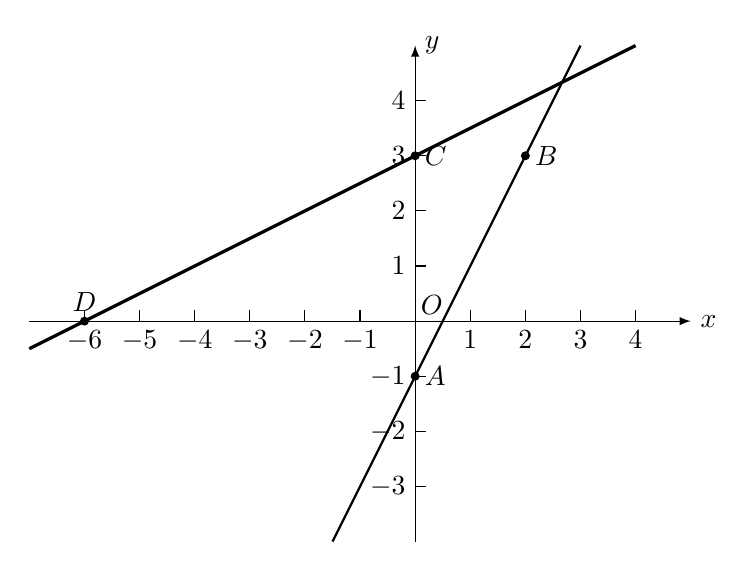
\begin{tikzpicture}[>=latex, scale=.7]
    \draw[->] (-7,0)--(5,0)node[right]{$x$};
    \draw[->] (0,-4)--(0,5)node[right]{$y$};
    \draw [domain =-1.5:3, samples=10, thick]plot(\x,{2*\x-1});
\draw [domain =-7:4, samples=10, very thick]plot(\x,{.5*\x+3});

\foreach \x in {-6,-5,...,-1,1,2,...,4}
{
    \draw (\x,0)node[below]{$\x$}--(\x,.2);
}
\foreach \x in {-3,-2,-1,1,2,3,4}
{
    \draw (0,\x)node[left]{$\x$}--(.2,\x);
}
\node at (.3,.3){$O$};
\draw (0,-1) [fill=black] circle (2pt)node[right]{$A$};
\draw (2,3) [fill=black] circle (2pt)node[right]{$B$};
\draw (0,3) [fill=black] circle (2pt)node[right]{$C$};
\draw (-6,0) [fill=black] circle (2pt)node[above]{$D$};
\end{tikzpicture}    
    \caption{}
\end{figure}
\end{solution}

\begin{ex}
\begin{enumerate}
    \item \begin{enumerate}
        \item 对于同一坐标系画出下列直线:
\[y=\frac{1}{2}x+4,\quad y=\frac{1}{2}-4,\quad y=-\frac{1}{2}x+4,\quad y=-\frac{1}{2}-4\]
\item 求每一条直线的斜率和在$y$轴上的截距.
\item 设$y=3$, 求各式中$x$的对应值,再用图象检验所得
结果.
    \end{enumerate}
    \item 作下列各直线:
\begin{multicols}{2}
    \begin{enumerate}
        \item $y=\frac{2}{3}x-5$
        \item $y=-3x+5$
        \item $y=-\frac{1}{2}x-\frac{9}{2}$
        \item $y=\frac{3}{4}x$
        \item $3x-5y=15$
        \item $x+2y+6=0$
    \end{enumerate}
\end{multicols}

\item \begin{enumerate}
    \item 已知一次函数$y=kx+b$在$x=-4$时,$y=9$, 在$x=6$
时,$y=3$, 求$k$和$b$.
\item 已知直线$y=kx+b$经过$(-4,9)$和$(6,3)$, 求$k$和$b$.
\end{enumerate}

\item 已知$y+b$与$x+a$成正比,$a,b$是常数,求证$y$是$x$的一次
函数,如果$x=3$时,$y=5$; $x=2$时,$y=2$, 求出表
示$y$是$x$的函数的解析式.
\item 直线$y=k_1x+b_1$和$y=k_2x+b_2$相交于$x$轴上同一点
$A(a,0)$, 求证在两直线上横坐标相同的点的纵坐标成正
比例变化.
\end{enumerate}
\end{ex}

\subsection{一次函数的性质}
我们在前面的内容中,曾直观地描述过函数的递增性和递减
性,当时是这样说的:“如果函数的值随着自变量的值增加而
增加,那么这个函数叫做\textbf{递增函数};如果函数的值随着自
变量的值增加而减少,那么这个函数叫做\textbf{递减函数}”.

现在让我们用较精确的语言,再来描述一下这个概念.

如果对于开区间$(a,b)$(或者闭区间$[a,b]$)上的任意两
个自变量的值$x_1$和$x_2$, 若
$x_1<x_2$,
则
$f(x_1)<f(x_2)$, 
那么函数$f(x)$称为在开区间$(a,b)$(或者闭区间$[a,b]$)上的
递增函数(图4.21).
\begin{figure}[htp]
    \centering
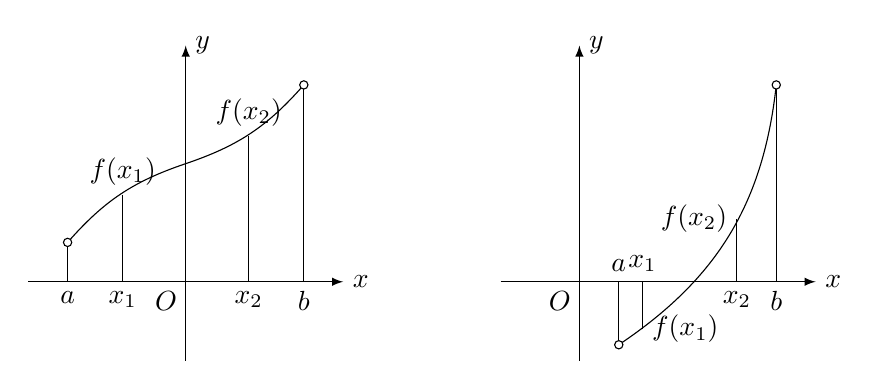
\begin{tikzpicture}[>=latex]
\begin{scope}
\draw[->](-2,0)--(2,0)node[right]{$x$};  
\draw[->](0,-1)--(0,3)node[right]{$y$};

\draw (-1.5,.5) to [bend left=15] (0,1.5) to [bend right=15] (1.5,2.5);
\draw (-1.5,.5)--(-1.5,0)node[below]{$a$};
\draw (1.5,2.5)--(1.5,0)node[below]{$b$};

\draw (-1.5,.5) [fill=white]circle(1.5pt) ;
\draw (1.5,2.5) [fill=white]circle(1.5pt) ;

\draw (-.8,1.1)node[above]{$f(x_1)$}--(-.8,0)node[below]{$x_1$};
\draw (.8,1.85)node[above]{$f(x_2)$}--(.8,0)node[below]{$x_2$};
\node at (-.25,-.25){$O$};
\end{scope}
\begin{scope}[xshift=5cm]
    \draw[->](-1,0)--(3,0)node[right]{$x$};  
\draw[->](0,-1)--(0,3)node[right]{$y$};
\draw (.5,-.8) to [bend left=-25] (2.5,2.5);
\draw (.5,-.8)--(.5,0)node[above]{$a$};
\draw (2.5,2.5)--(2.5,0)node[below]{$b$};
\node at (-.25,-.25){$O$};


\draw (.8,-.6)node[right]{$f(x_1)$}--(.8,0)node[above]{$x_1$};
\draw (2,.8)node[left]{$f(x_2)$}--(2,0)node[below]{$x_2$};
\draw (.5,-.8) [fill=white]circle(1.5pt) ;
\draw (2.5,2.5) [fill=white]circle(1.5pt) ;
\end{scope}    
\end{tikzpicture} 
\caption{}
\end{figure}


如果对于开区间$(a,b)$(或者闭区间$[a,b]$)上的任意两
个自变量的值$x_1$和$x_2$,若
$x_1<x_2$,
则
$f(x_1)>f(x_2)$,
那么函数$f(x)$称为在开区间$(a,b)$(或者闭区间$[a,b]$)上的
递减函数(图4.22).

\begin{figure}[htp]
    \centering
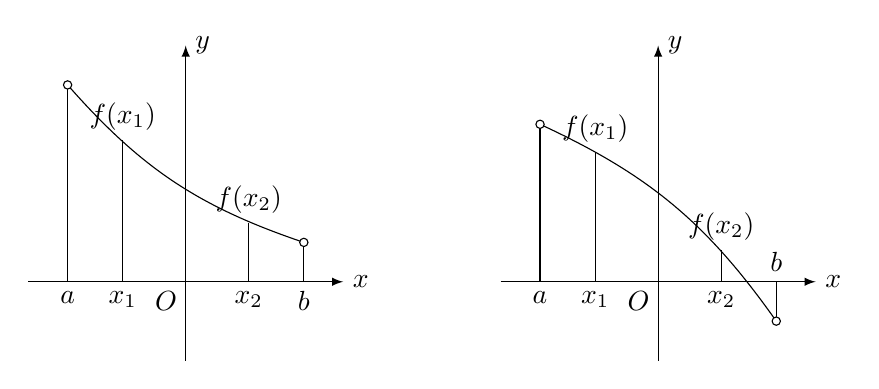
\begin{tikzpicture}[>=latex]
\begin{scope}
    \draw[->](-2,0)--(2,0)node[right]{$x$};  
\draw[->](0,-1)--(0,3)node[right]{$y$};
\node at (-.25,-.25){$O$};
\draw (-1.5,2.5) to [bend left=-15] (1.5,.5);
\draw (-1.5,2.5)--(-1.5,0)node[below]{$a$};
\draw (1.5,.5)--(1.5,0)node[below]{$b$};

\draw (-.8,1.8)node[above]{$f(x_1)$}--(-.8,0)node[below]{$x_1$};
\draw (.8,.75)node[above]{$f(x_2)$}--(.8,0)node[below]{$x_2$};




\draw (-1.5,2.5) [fill=white]circle(1.5pt) ;
\draw (1.5,.5) [fill=white]circle(1.5pt) ;
\end{scope}
\begin{scope}[xshift=6cm]
    \draw[->](-2,0)--(2,0)node[right]{$x$};  
    \draw[->](0,-1)--(0,3)node[right]{$y$};
    \node at (-.25,-.25){$O$};
    \draw (-1.5,2) to [bend left=15] (1.5,-.5);
    \draw (-1.5,2)--(-1.5,0)node[below]{$a$};
    \draw (1.5,-.5)--(1.5,0)node[above]{$b$};
    \draw (-.8,1.65)node[above]{$f(x_1)$}--(-.8,0)node[below]{$x_1$};
    \draw (.8,.4)node[above]{$f(x_2)$}--(.8,0)node[below]{$x_2$};
    

    \draw (-1.5,2) [fill=white]circle(1.5pt) ;
    \draw (1.5,-.5) [fill=white]circle(1.5pt) ;  
\end{scope}    
\end{tikzpicture} 
\caption{}
\end{figure}

下面我们来阐明一次函数$y=kx+b$的增减性,当$k>0$
时,一次函数$y=kx+b$在定义域上是递增的;当$k<0$时,
一次函数$y=kx+b$在定义域上是递减的.现在证明上述结
论:

在定义域中任取两数$x_1,x_2$且$x_1<x_2$, 那么
\[y_2-y_1=(kx_2+b)-(kx_1+b)=k(x_2-x_1)\]
因$x_1<x_2$, 即$x_2-x_1>0$, 故:
\begin{itemize}
    \item 若$k>0$, 则$k(x_2-x_1)>0$, 即$y_2>y_1$, 所以$y=kx+b$
是递增的.
\item 若$k<0$, 则$k(x_1-x_2)<0$, 即$y_1<y_2$, 所以$y=kx+b$
是递减的.
\end{itemize}

下面我们来研究一次函数的变化率:

设函数$y=kx+b$的自变量从$x_1$变到$x_2$, 因变量则从$y_1$变
到$y_2$. 设$\Delta x=x_2-x_1$为自变量的改变量,$\Delta y=y_2-y_1$为因变
量的改变量.我们称函数改变量与自变量改变量的比
$\frac{\Delta y}{\Delta x}$
为函数$y$对于自变量$x$的\textbf{平均变化率}.

由$y_1=kx_1+b$和$y_2=kx_2+b$得:$y_2-y_1=k(x_2-x_1)$,即:
\[\Delta y=k\Delta x\]
这表示一次函数的改变量与自变量的改变量成正比例变化,
比例常数$k$就是一次函数的斜率,因此
\[\frac{\Delta y}{\Delta x}=k\]
即一次函数的变化率总是常数,等于一次函数的斜率$k$(图
4.23).

\begin{figure}[htp]
    \centering
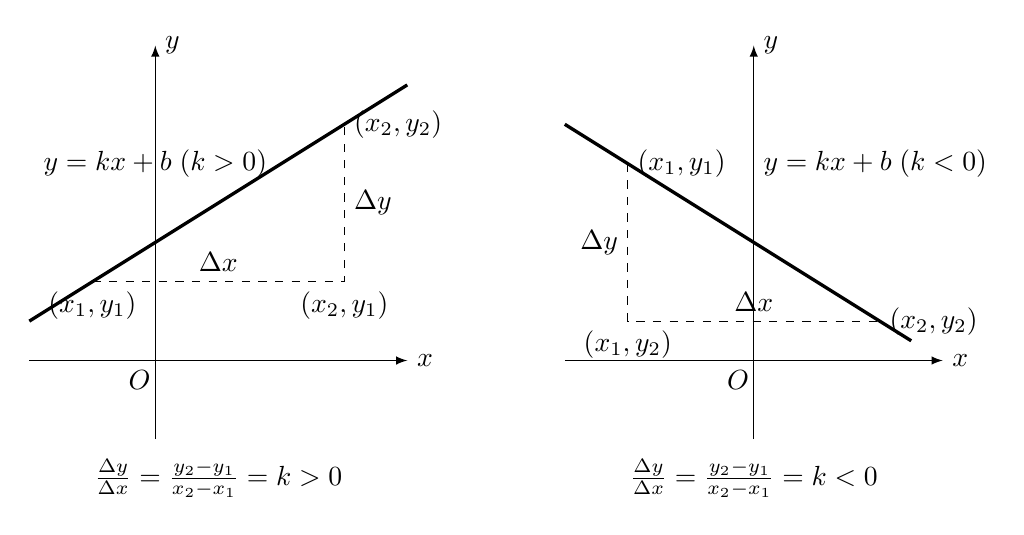
\begin{tikzpicture}[>=latex, xscale=.8, yscale=1]
\begin{scope}
    \draw[->](-2,0)--(4,0)node[right]{$x$};  
    \draw[->](0,-1)--(0,4)node[right]{$y$};
    \node at (-.25,-.25){$O$};
\draw [domain=-2:4, samples=10, very thick] plot(\x, {0.5*\x+1.5});
\draw[dashed](-1,1)node[below]{$(x_1,y_1)$}--node[above]{$\Delta x$}(3,1)node[below]{$(x_2,y_1)$}--node[right]{$\Delta y$}(3,3)node[right]{$(x_2,y_2)$};
\node at (0,2.5){$y=kx+b\; (k>0)$};
\node at (1,-1.5){$\frac{\Delta y}{\Delta x}=\frac{y_2-y_1}{x_2-x_1}=k>0$};

\end{scope}
\begin{scope}[xshift=9.5cm]
    \draw[->](-3,0)--(3,0)node[right]{$x$};  
    \draw[->](0,-1)--(0,4)node[right]{$y$};
    \node at (-.25,-.25){$O$};
    \draw [domain=-3:2.5, samples=10, very thick] plot(\x, {-0.5*\x+1.5});
    \draw[dashed](-2,2.5)node[right]{$(x_1,y_1)$}--node[left]{$\Delta y$}(-2,.5)node[below]{$(x_1,y_2)$}--node[above]{$\Delta x$}(2,.5)node[right]{$(x_2,y_2)$};
    \node at (0,2.5)[right]{$y=kx+b\; (k<0)$};
    \node at (0,-1.5){$\frac{\Delta y}{\Delta x}=\frac{y_2-y_1}{x_2-x_1}=k<0$};
\end{scope}
\end{tikzpicture}    
    \caption{}
\end{figure}

变化率为常数说明:
\begin{enumerate}
    \item 不管$x_1,x_2$在区间的什么位置,
即$\Delta x$不管在何处产生,变化率$\frac{\Delta y}{\Delta x}$
是一样的;
\item 变化时时
刻刻在发生,不管$\Delta x$多小,变化率也是一样的,这就表明,
函数$y$随着$x$而均匀变化.
\end{enumerate}

反过来看,如果一个函数的平均变化率等于一个常量$k$, 
那么这个函数是一次函数.

事实上,任意取定函数$y=f(x)$的一对对应值$x_1$和$y_1=
f(x_1)$, 设$\Delta x=x-x_1$, $\Delta y=y-y_1$, 因为函数$y=f(x)$的变
化率等于常数$k$, 因此有
\[\frac{\Delta y}{\Delta x}=k\]
即
\[\frac{y-y_1}{x-x_1}=k\]
化简得
\[y=kx-kx_1+y_1\]
也即:$y=kx+b$, 这里$b=-kx_1+y_1$(常数).

因此函数$y=f(x)$是$x$的一次函数.    

\begin{example}
    一定量的酒精,在温度$t=0^{\circ}{\rm C}$时,体积$V=5.25$升,实验表明,温度每升高$10^{\circ}{\rm C}$, 体积增大0.06升,求体积$V$与温度$t$的变化关系.
\end{example}    

\begin{solution}
因为这里体积的增量与温度的增量成正比:
$\frac{\Delta V}{\Delta t}= 0.006$, 所以$V$与$t$的关系可表为一次函数$V=0.006t+b$, 只
    需要再确定常数$b$.

    因为$t=0$时,$V=5.25$, 所以有
   \[ 5.25=0.006\x 0+b\quad \Rightarrow\quad b=5.25\]
   故所求函数关系是$V=0.006t+5.25$.
\end{solution}


\section*{习题4.3}
\addcontentsline{toc}{subsection}{习题4.3}
\begin{enumerate}
\item 试证正比例函数$y=kx$, 当$k>0$时,在定义域上是递
增的,当$k<0$时,在定义域上是递减的.

\item 试证反比例函数$y=\frac{k}{x}$,
当$k>0$时,在$(0,+\infty)$上是
递减的,当$k<0$时,在$(0,+\infty)$上是递增的.
\item  \begin{enumerate}
    \item 对于同一坐标系,作函数$y=3x+2$和$y=-3x+2$
的图象.
\item 所得的两个图象有哪些相同的地方?有哪些不同的
地方?
\item 求证:$x$的值每次增加一个相同的数,函数$y=3x+2$
的值也每次增加一个相同的数,而函数$y=-3x-2$的
值却每次减少一个相同的数.
\item 求证:函数$y=3x+2$所增加的量和对应的自变量
$x$所增加的量的比等于3, 而对于函数$y=-3x+2$,
这个比等于$-3$.
\end{enumerate} 

\item 
在匀速运动中,某物体所行路程与行动时间的关系由
关系式$s=2t+40$表示.$t$与$s$的大小是成正比例吗?如
果$s$的单位是米,$t$的单位是秒,问每经过一秒这物体就
前进多少米?
\item 
中夜的气温是$5^{\circ}$C,到明天下午2时以前气温按每小时$0.2^{\circ}$C均匀地升高,用公式表示气温$y$与时间$x$的函数关系,写出这函数的定义域.

\item 弹簧的原长3厘米,在由0.5(kg)到3.5(kg)的载重限
度内,每加重一千克弹簧伸长0.5毫米,用公式表示弹
簧长度与载重量间的函数关系.这函数的定义域是什么?
\item 钢杆由于温度上升$1^{\circ}$C所增加的长度和$0^{\circ}$C时的长度比
等于0.000011每度,用公式表示钢杆在$t^{\circ}$C时的长度与温
度$t$的函数关系.
\item 钢桥在$0^{\circ}$C时的长度是400米.求温度从$-20^{\circ}$C上升到
$40^{\circ}$C时钢桥的长度变化了多少?
\item 当压强不变时,一切气体的体积由于温度上升$1^{\circ}$C所增加的体积和$0^{\circ}$C时的气体的体积的比大致是相等的,并等于$\frac{1}{273}$每度.
这就是盖吕萨克定律,写出在$t^{\circ}$C时的体积$v$和温度$t$的函数关系.

\end{enumerate}

\subsection{方程$ax+by+c=0$的图象}
在前面的内容中,我们已经知道函数$y=kx+b\; (k\ne 0)$的图象
是一条直线,但是无论$k$和$b$取什么数值,一次函数的图象仅
是坐标平面上直线集合中的一部分,因为$k\ne 0$, 所以直线
$y=kx+b\; (k\ne 0)$, 不能表示$x$轴以及和$x$轴平行的任何直线.
又当直线向上方向与$x$轴正方向所成角$\alpha=90^{\circ}$时,$k=\tan\alpha$不存
在,这就是说直线$y=kx+b\; (k\ne 0)$, 不能表示$y$轴以及和$y$
轴平行的直线.我们把函数关系$y=kx+b$, 也可以看做是关
于$x$和$y$的一次方程
\[kx-y+b=0\]
这样,我们也就可以知道二元一次方程
\[kx-y+b=0\]
的图象是一条直线.

现在,我们来研究一般的情况,证明任何一个二元一次
方程
\[ax+by+c=0\qquad  \text{($a,b$不同时为零)}\]
的图象都是直线.

根据$a,b$可取值的条件,可以看出要证明这个结论应该
分三种情况,就是:
\begin{itemize}
    \item $a\ne 0,\quad b\ne 0$
    \item $a=0,\quad b\ne 0$
    \item $a\ne 0,\quad  b=0$
\end{itemize}

\begin{enumerate}
    \item $a\ne 0,b\ne 0$, 这时方程可以化为:
    \begin{equation}
        y=-\frac{a}{b}x-\frac{c}{b}
    \end{equation}
这是$x$的一次函数,我们已经知道它的图象是一条直线,这条
直线的斜率是$-\frac{a}{b}$,
在$y$轴上的截距是$-\frac{c}{b}$.如果$c=0$, 那
么这条直线就经过原点.

\item $a=0,b\ne 0$, 这时方程可化为:
\begin{equation}
    y=0x-\frac{c}{b}
\end{equation}
这里可以看到,不论变量$x$取什么实数值,和它对应的$y$的值
总等于$-\frac{c}{b}$.
所以它的图象是平行于$x$轴,并且和$x$轴的距离等
于$-\frac{c}{b}$的直线.当$-\frac{c}{b}>0$时,直线在$x$轴上方;当$-\frac{c}{b}<0$时,直线在$x$轴下方,特别,当$c=0$时,$-\frac{c}{b}=0$, 这时
$y=0$, 它的图象就是$x$轴(图4.24).

\item $a\ne 0,b=0$, 这时方程可化为:
\begin{equation}
    x=0\cdot y-\frac{c}{a}
\end{equation}

可以看到,不论变量$y$取什么数值,和它对应的$x$的值总
等于$-\frac{c}{a}$.
所以它的图象是平行$y$轴,并且和$y$轴的距离是
$-\frac{c}{a}$的一条直线.当$-\frac{c}{a}>0$
时,直线在$y$轴的右边,当
$-\frac{c}{a}<0$时,直线在$y$轴的左边,特别,当$c=0$时,$-\frac{c}{a}=0$,
这时$x=0$, 它的图象就是$y$轴(图4.25).

\begin{figure}[htp]\centering
    \begin{minipage}[t]{0.48\textwidth}
    \centering
    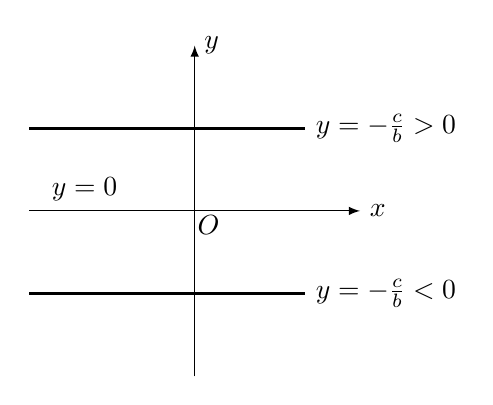
\begin{tikzpicture}[>=latex, scale=.7]
        \draw[->](-3,0)--(3,0)node[right]{$x$};
        \draw[->] (0,-3)--(0,3)node[right]{$y$};
    \draw[very thick] (-3,1.5)--(2,1.5)node[right]{$y=-\frac{c}{b}>0$};
    \draw[very thick] (-3,-1.5)--(2,-1.5)node[right]{$y=-\frac{c}{b}<0$};
    \node at (-2,0)[above]{$y=0$};
    \node at (.25,-.25){$O$};
    \end{tikzpicture}
    \caption{}
    \end{minipage}
    \begin{minipage}[t]{0.48\textwidth}
    \centering
    \begin{tikzpicture}[>=latex, scale=.7]
        \draw[->](-3,0)--(3,0)node[right]{$x$};
        \draw[->] (0,-3)--(0,3)node[right]{$y$};
        \node at (.25,-.25){$O$};
        \draw[very thick] (1.5,-3)--(1.5,3)node[right]{$x=-\frac{c}{a}>0$};
        \draw[very thick] (-1.5,-3)--(-1.5,3)node[left]{$x=-\frac{c}{a}<0$};
\node at  (0,-3)[fill=white]{$x=0$};
    \end{tikzpicture}
    \caption{}
    \end{minipage}
    \end{figure}
\end{enumerate}

总结上面这三种情况,我们得到:
方程$ax+by+c=0$ ($a,b$不同时等于零)的图象是一条直
线.

以后我们把这个图象,简称为直线$ax+by+c=0
$.



\begin{example}
    在同一坐标系里作以下方程的图象:
\[x-y+2=0,\qquad 2x+y+1=0\]
\end{example}

\begin{solution}
列表:
\begin{multicols}{2}
    \begin{center}
        \begin{tabular}{c|cc}
           \hline
            $x$&0&$-2$\\
            \hline
            $y$&2&0\\
            \hline
        \end{tabular}
    \end{center}
    \begin{center}
        \begin{tabular}{c|cc}
            \hline
            $x$&0&$-\frac{1}{2}$\\
            \hline
            $y$&$-1$&0\\
            \hline
        \end{tabular}
    \end{center}
\end{multicols}
图象如图4.26

\begin{figure}[htp]
    \centering
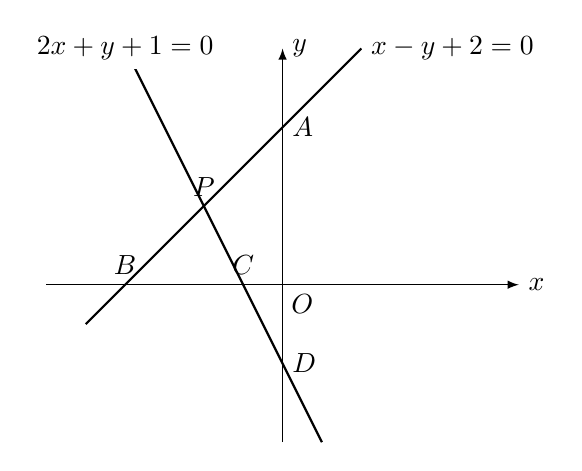
\begin{tikzpicture}[>=latex]
\draw[->] (-3,0)--(3,0)node[right]{$x$};
\draw[->] (0,-2)--(0,3)node[right]{$y$};
\node at (.25,-.25){$O$};    
\draw [domain=-2.5:1, samples=10, thick]plot(\x, {\x+2});
\draw [domain=-2:.5, samples=10, thick]plot(\x, {-1-2*\x});
\node at (-2,3)[fill=white]{$2x+y+1=0$};
\node at (1,3)[fill=white, right]{$x-y+2=0$};
\node at (0,2)[right]{$A$};\node at (0,-1)[right]{$D$};
\node at (-2,0)[above]{$B$};
\node at (-.5,0)[above]{$C$};
\node at (-1,1)[above]{$P$};

\end{tikzpicture}
    \caption{}
\end{figure}

如果在同一坐标系要画出二元一次方程组里两个方程的
图象,就可以根据图象求出方程组的解.这种解法叫做二元
一次方程组的图象解法.现在举例说明如下:
\end{solution}

\begin{example}
    用图象法解方程组:
    \begin{numcases}{}
        x-y+2=0\\
        2x+y+1=0
    \end{numcases}
\end{example}

\begin{solution}
在例4.17里我们已经画过这两个方程的图象,它们是
两条相交直线$AB$和$CD$(图4.26),这个交点$P$的坐标是$x=-1$, $y=1$, 它就是所求方程组的解.

这是因为$P$点既在方程(4.6)的图象$AB$上,又在方程(4.7)
的图象$CD$上,所以它的坐标$x=-1$, $y=1$, 既适合方程
(4.6)又适合方程(4.7),因此$x=-1$, $y=1$是方程组的解.

反过来,方程组的解,必须同时适合方程(4.6)和(4.7),
所以表示它的点必须既在方程(4.6)的图象$AB$上,又在方程
(4.7)的图象$CD$上,因此它必须是$AB$和$CD$的交点$P$.这就是
说,除去$x=-1$, $y=1$以外,方程组不再有其它的解.

\end{solution}

\begin{example}
    用图象法解下面的方程组:
    \begin{numcases}
    2x-3y+4=0\\
    4x-6y+8=0        
    \end{numcases}
\end{example}


\begin{solution}
 列表
 \begin{multicols}{2}
    \begin{center}
        \begin{tabular}{c|cc}
           \hline
            $x$&1&$-2$\\
            \hline
            $y$&2&0\\
            \hline
        \end{tabular}
    \end{center}
    \begin{center}
        \begin{tabular}{c|cc}
            \hline
            $x$&1&$-2$\\
            \hline
            $y$&$2$&0\\
            \hline
        \end{tabular}
    \end{center}
\end{multicols}

\begin{figure}[htp]
    \centering
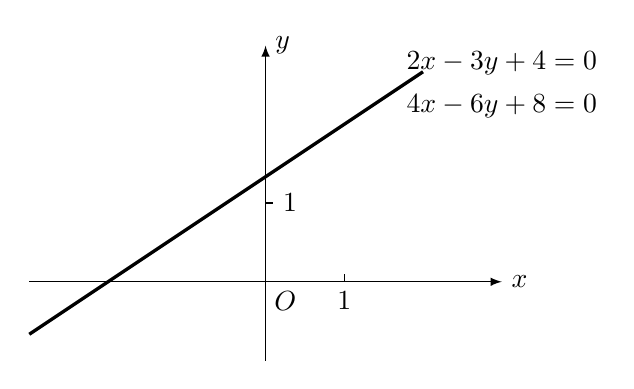
\begin{tikzpicture}[>=latex]
    \draw[->] (-3,0)--(3,0)node[right]{$x$};
    \draw[->] (0,-1)--(0,3)node[right]{$y$};
    \node at (.25,-.25){$O$};   
\draw[domain=-3:2, samples=10, very thick]plot (\x, {2*\x/3+4/3});
\node at (3,2.5)[below]{$4x-6y+8=0$};
\node at (3,2.5)[above]{$2x-3y+4=0$};
\draw (1,0)node[below]{1}--(1,.1);
\draw (0,1)--(.1,1)node[right]{1};

\end{tikzpicture}
    \caption{}
\end{figure}

    这两个方程的图象是同一条直线(图4.27),所以在直线
    上的每一个点的坐标都是这两个方程的公共解,方程组有无
    穷多解.     
\end{solution}



\begin{example}
    用图象法解下面的方程组:
\begin{numcases}{}
    2x-3y+4=0\\
    4x-6y-2=0
\end{numcases}
\end{example}

\begin{solution}
    列表
    \begin{multicols}{2}
       \begin{center}
           \begin{tabular}{c|cc}
              \hline
               $x$&1&$-2$\\
               \hline
               $y$&2&0\\
               \hline
           \end{tabular}
       \end{center}
       \begin{center}
           \begin{tabular}{c|cc}
               \hline
               $x$&$-1$&2\\
               \hline
               $y$&$-1$&1\\
               \hline
           \end{tabular}
       \end{center}
   \end{multicols}
   \begin{figure}[htp]
    \centering
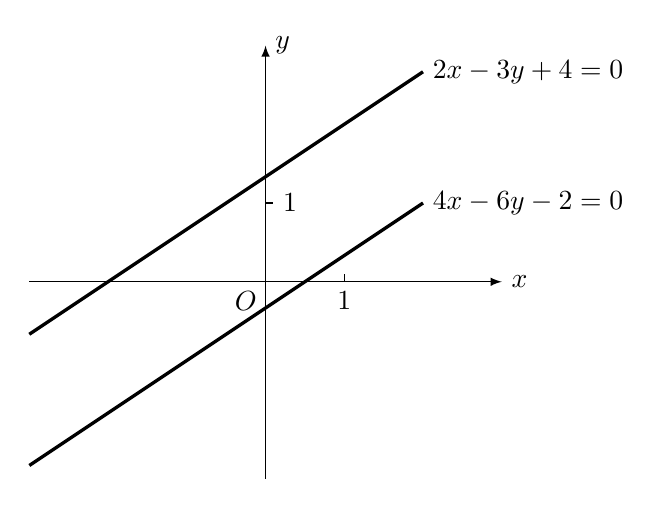
\begin{tikzpicture}[>=latex]
    \draw[->] (-3,0)--(3,0)node[right]{$x$};
    \draw[->] (0,-2.5)--(0,3)node[right]{$y$};
    \node at (-.25,-.25){$O$};   
\draw[domain=-3:2, samples=10, very thick]plot (\x, {2*\x/3+4/3});
\draw[domain=-3:2, samples=10, very thick]plot (\x, {2*\x/3-1/3});
\node at (2,8/3)[right]{$2x-3y+4=0$};
\node at (2,1)[right]{$ 4x-6y-2=0$};
\draw (1,0)node[below]{1}--(1,.1);
\draw (0,1)--(.1,1)node[right]{1};

\end{tikzpicture}
    \caption{}
\end{figure}

由图4.28看出,当两条直线方程的斜率相同而截距不同
时,这两个方程的图象是两条互相平行的直线,它们没有公
共的点,所以这个方程组没有解.
\end{solution}


从例4.18、4.19、4.20可以知道,二元一次方程组的解可以有三种情况:
\begin{enumerate}
   \item 有一组且只有一组解(方程组里两个方程的图象是
两条相交直线)、
\item 有无穷多组解(方程组里两个方程的图象是同一条
直线).
\item 没有解(方程组里两个方程的图象是两条互相平行
的直线). 
\end{enumerate}

因为平面上两条直线的相互位置关系,只有相交、重
合、平行这三种情况,所以二元一次方程组的解,也只可能
有这三种情况.

\section*{习题4.4}
\addcontentsline{toc}{subsection}{习题4.4}
\begin{enumerate}
    \item 
    求作下列各方程的图象:
\begin{multicols}{2}
\begin{enumerate}
    \item $3x+2y=6$
    \item $4x+6y+9=0$
    \item $3y-4=5x$
    \item $x+y=0$
    \item $3x-4y=0$
\end{enumerate}
\end{multicols}
 
 \item 对于同一坐标系,作下列各方程的图象:
 \begin{multicols}{2}
    \begin{enumerate}
        \item $y=2$
        \item $y=-2$
        \item $x=4$
        \item $x=-4$
        \item $x=0$
        \item $y=0$
    \end{enumerate}
    \end{multicols}
\item \begin{enumerate}
   \item 已知函数$y=3x-2$和$y=2x+3$, 求作这两个函
    数的图象;
    \item 根据这两个图象,求$x$等于什么数值的时候,函数$y=3x-2$和$y=2x+3$有相同的值;
    \item 用图象法解方程$6x+3=4x-7$. 
\end{enumerate}

\item     用图象法解下列各方程组:
  \begin{multicols}{2}
\begin{enumerate}
    \item $\begin{cases}
        y=-\frac{2}{3}x+5\\
        y=\frac{3}{2}x-8
    \end{cases}$
    \item $\begin{cases}
        x+y=5\\x-y=1
    \end{cases}$
    \item $\begin{cases}
        3x+y=9\\x+2y=-2
    \end{cases}$
    \item $\begin{cases}
        2x-5y+16=0\\3x+4y+1=0
    \end{cases}$
\end{enumerate}
\end{multicols}
    \item 讨论下列各方程组的解,并且用图象表示出来:
    \begin{multicols}{2}
        \begin{enumerate}
\item $\begin{cases}
    x-y-5=0\\2x+2y-9=0
\end{cases}$    
\item $\begin{cases}
     x+y=3\\2x+2y=7
\end{cases}$ 
\item $\begin{cases}
    x-3y+2=0\\3x-9y+6=0
\end{cases}$ 
\item $\begin{cases}
    x-4=y\\2x-2y=5
\end{cases}$ 
        \end{enumerate}
\end{multicols}
   
\item 四条直线:$2x+y=6$, $x+2y=6$, $x$轴和$y$轴围成-个四边形,求这四边形的面积.

\end{enumerate}

\subsection{二元一次不等式的图象}
前面我们已经研究过$ax+by+c=0$ ($a,b$不同时为零)
的图象是这样一条直线,它上面的点的坐标是适合方程的所
有有序对$(x,y)$的集合.

现在来研究$ax+by+c>0$或$ax+by+c<0$($a,b$不同时
为零)的图象,类似上面这种含有二个一次变数的不等式叫做
二元一次不等式,使二元一次不等式成立的有序实数对$(x,y)$
叫做 二元一次不等式的解.例如:
\begin{equation}
 3x+y+5>0   
\end{equation}
对于$(-3,5)$有$3\x(-3)+5+5=
1>0$, (4.12)成立,因此$(-3,5)$是它的解,又$(-5,7)$
使$3(-5)+7+5=-3<0$, 所以$(-5,7)$不是(4.12)
的解.

根据图象的意义,$ax+by+c>0$ (或$<0$) (这里$a^2+b^2>
0$) 的图象就是所有适合$ax+by+c>0$ (或$<0$) 的有序对的
集合,以这样的有序对为坐标的所有点的集合表示平面上的
什么图形呢?我们从一个具体例子入手,看看$3x-y+5>0$
的图象是什么,也就是要看看$y<3x+5$的图象是什
么?

现在在直线$y=3x+5$上取一点,若$x=1$则$y=8$. 因此
$A(1,8)$是在直线$y=3x+5$上的点,如果在点$A$的正下方取
点$A_1,A_2,\ldots$, 因为这些点的$x$坐标仍为1, 但$y$的坐标小于
8, 这样把$x=1$与小于8的任意的$y$配对,如$(1,7)$, 
$\left(1,\frac{15}{2}\right)$, $(1,-2000),\ldots$都适合$y<3x+5$, 因此都
是$y<3x+5$图象上的点,再在点
$A$的正上方取某些点,则这
些点的坐标不适合$y<3x+5$.同样,在直线$y=3x+5$上另
取一点$B(-2,-1)$, 这样把$x=-2$与小于$-1$的任意
$y$配对都是$y<3x+5$图象上的点,而把$x=-2$与大于$-1$
的任意$y$配对就都不适合$y<3x+5$, 由此可见,$y=3x+5$的
图象是过$A,B$的一条直线,而$y<3x+5$的图象是以直线
$AB$为界的开的半平面(不包括直线$AB$),如图4.29中的阴影部分.

\begin{figure}[htp]
    \centering
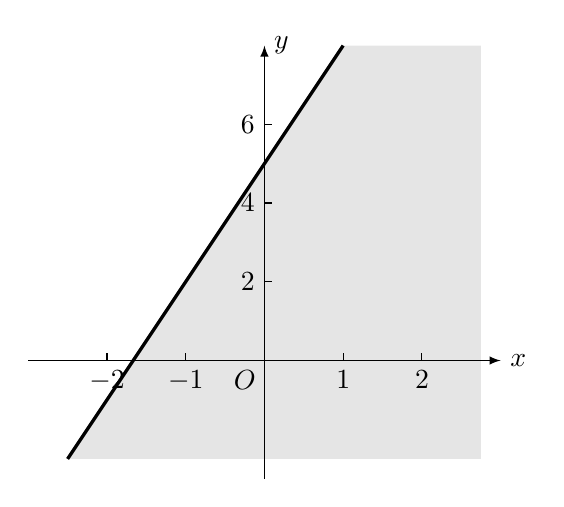
\begin{tikzpicture}[>=latex, yscale=.5]
\fill [gray!20] (-2.5,-2.5)--(1,8)--(2.75,8)--(2.75,-2.5)--(-2.5,-2.5); 
   \draw[->] (-3,0)--(3,0)node[right]{$x$};
    \draw[->] (0,-3)--(0,8)node[right]{$y$};
    \node at (-.25,-.5){$O$};   
\foreach \x in {-2,-1,1,2}
{
    \draw (\x,0)node[below]{$\x$}--(\x,.2);
}
\draw [domain=-2.5:1, samples=10, very thick] plot(\x, {3*\x+5});
\foreach \y in {2,4,6}
{
    \draw (0,\y)node[left]{$\y$}--(.1,\y);
}

\end{tikzpicture}
    \caption{}
\end{figure}

现在的问题是,直
线$3x-y+5=0$把平
面分成除直线外的两个
半平面,$3x-y+5>0$
表示两个半平面之一,
我们如何较方便地而不
必把不等式就$y$来解就
可以确定$3x-y+5>0$
是哪个半平面?这是非
常容易确定的,因为
$3x-y+5>0$所确定的
那个半平面内,一切点的坐标都满足$3x-y+
5>0$. 故我们只要任意选一点,譬如说原点$(0,0)$, 把它
代到$3x-y+5$中,如果结果大于零,那么$3x-y+5>0$
就是包含原点的那个平面,不然就是不包含原点的那个平面,
现在实际代入的结果$3\x0-0+5>0$, 故$3x-y+5>0$的
图象就是包含原点的那个半平面了,另一个半平面就是
$3x-y+5<0$的图象了.二元一次不等式的图象也叫做不等
式的表示区域.

\begin{example}
图示下列不等式组的图象:
\[\begin{cases}
  2x+3y-6\ge 0\\
2x-3y-6\le 0 
\end{cases}\]
 \end{example}

\begin{solution} 
$2x+3y-6\ge 0$的图象是以直线$m:\; 2x+3y-6=0$
为界包括$m$不含$(0,0)$的半平面;
$2x-3y-6\le 0$的图象是以直线$h:\; 2x-3y-6=0$为
界包括$h$包含$(0,0)$的半平面.不等式组的解集的图象是这
两个半平面的公共部分.换言之,不等式组的解集图象是这个
不等式组中各个不等式图象的交集(图4.30).

\begin{figure}[htp]
    \centering
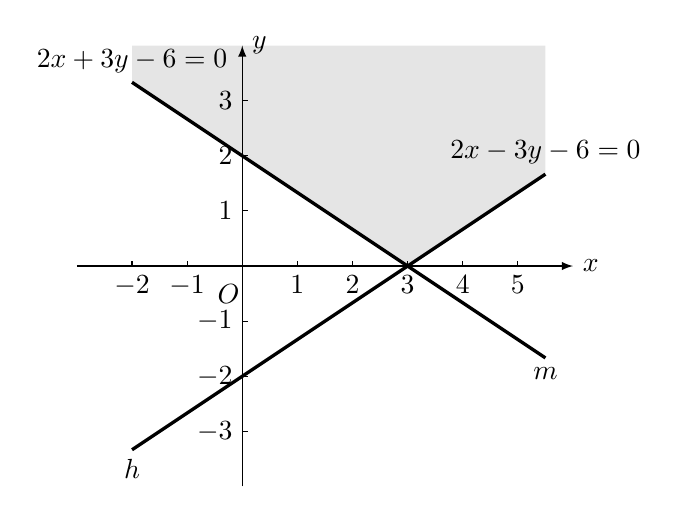
\begin{tikzpicture}[>=latex, scale=.7]
\fill [gray!20](-2,10/3)node[above, black]{$2x+3y-6= 0$}--(-2,4)--(5.5,4)--(5.5,5/3)node[above, black]{$2x-3y-6= 0$}--(3,0)--(-2,10/3);
\node at (-2,-10/3) [below]{$h$};
\node at (5.5,-5/3) [below]{$m$};
    \draw[->] (-3,0)--(6,0)node[right]{$x$};
    \draw[->] (0,-4)--(0,4)node[right]{$y$};
    \node at (-.25,-.5){$O$};   
\foreach \x in {-2,-1,1,2,...,5}
{
    \draw (\x,0)node[below]{$\x$}--(\x,.1);
}
\draw [domain=-2:5.5, samples=10, very thick] plot(\x, {2-2*\x/3});
\draw [domain=-2:5.5, samples=10, very thick] plot(\x, {2*\x/3-2});

\foreach \y in {-3,-2,-1,1,2,3}
{
    \draw (0,\y)node[left]{$\y$}--(.1,\y);
}


\end{tikzpicture}
    \caption{}
\end{figure}
\end{solution}



\begin{example}
    图示不等式组的图象:
\[\begin{cases}
   x\ge  0\\
    y\ge -1\\
    x+y\le 3\\
    x\le 2
\end{cases}\]
\end{example}



\begin{solution}
不等式组的解集是由
四条直线所围成的,在图4.31
中阴影部分的四边形$ABCD$的
周界以及它的内部.因此不等
式组的图象是一个凸区域.
\end{solution}

我们已经知道二元一次不
等式组的解集的图象是一个凸
区域.是不是二元一次不等式组总表示一个凸区域呢?下面
的例子指出存在二元一次不等
式组不构成区城的情况.

\begin{example}
   不等式组:
   \[\begin{cases}
    y\ge 0\\
    x-y\ge 3\\
    5x+2y\le 10    
   \end{cases}\]
没有解. 
\end{example}

\begin{solution}
    因从图象上来看(图4.32),
对应于这三个不等式的半平面
没有公共部分.


\end{solution}

\begin{figure}[htp]\centering
    \begin{minipage}[t]{0.48\textwidth}
    \centering
    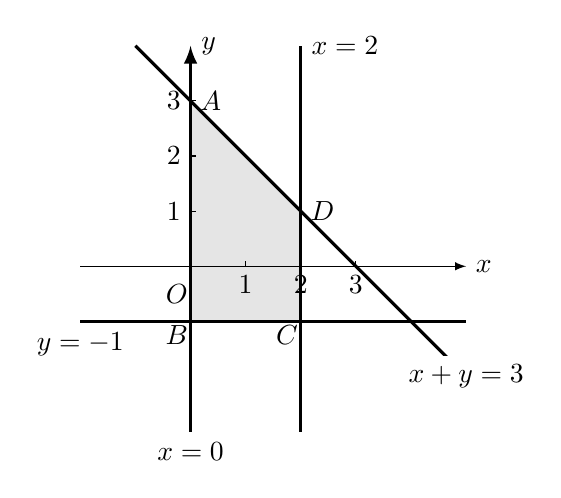
\begin{tikzpicture}[>=latex, scale=.7]
        \fill [gray!20](0,-1)--(2,-1)--(2,1)node[right, black]{$D$}--(0,3)node[right, black]{$A$}--(0,-1);
    
    
        \draw[->] (-2,0)--(5,0)node[right]{$x$};
        \draw[->,very thick] (0,-3)node[below]{$x=0$}--(0,4)node[right]{$y$};
        \node at (-.25,-.5){$O$};   
        \foreach \x in {1,2,3}
        {
            \draw (\x,0)node[below]{$\x$}--(\x,.1);
            \draw (0,\x)node[left]{$\x$}--(.1,\x);
        }
        \draw [domain=-1:5, samples=10, very thick] plot(\x, {3-\x});
        \draw[very thick] (-2,-1)node[below]{$y=-1$}--(5,-1);
        \draw[very thick] (2,-3)--(2,4)node[right]{$x=2$};
    \node at (5,-2) [fill=white]{$x+y=3$};
    \node at (0-.25,-1-.25){$B$};
    \node at (2-.25,-1-.25){$C$};
    \end{tikzpicture}
    \caption{}
    \end{minipage}
    \begin{minipage}[t]{0.48\textwidth}
    \centering
    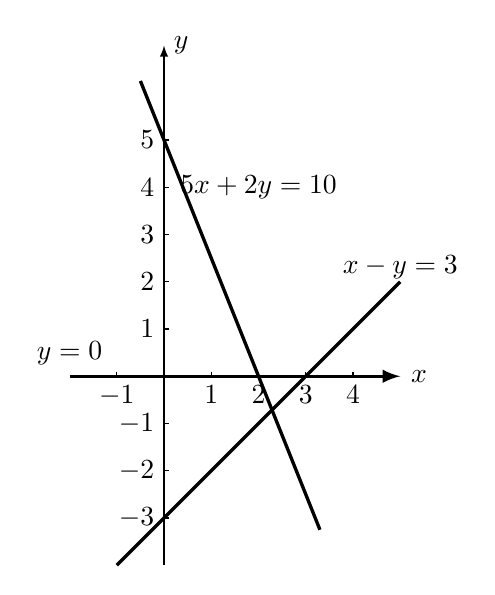
\begin{tikzpicture}[>=latex, scale=.6]
        \draw[->,very thick] (-2,0)node[above]{$y=0$}--(5,0)node[right]{$x$};
        \draw[->] (0,-4)--(0,7)node[right]{$y$};
        \foreach \x in {-1,1,2,...,4}
        {
            \draw (\x,0)node[below]{$\x$}--(\x,.1);
        }
    \foreach \y in {-3,-2,-1,1,2,...,5}
    {
        \draw (0,\y)node[left]{$\y$}--(.1,\y);
    }
    \draw [domain=-1:5, samples=10, very thick] plot(\x, {\x-3});
    \draw [domain=-.5:3.3, samples=10, very thick] plot(\x, {5-2.5*\x});
    
    \node at (2,4){$5x+2y=10$};
    \node at (5,2.3){$x-y=3$};
    
    \end{tikzpicture}
    \caption{}
    \end{minipage}
    \end{figure}



\begin{example}
    王明购买价格是3
角和5角的笔记本若干本,每
种至少买一本,但不得超过2.6元,问有多少种买法?指出正好花完2.6元的情形.
\end{example}

\begin{solution}
    设购买3角的笔记本$x$本,5角的笔记本$y$本,依题
意列出不等式组:
\[\begin{cases}
    0.3x+0.5y\le 2.6\\
x\ge 1\\
y\ge 1
\end{cases}\]
其中$x,y$是整数.

所以只要在$\triangle ABC$围成的凸区域,包括周界,数出坐标是整
数的点的个数即可,由图
4.33可以看出,这样的点
共17个,每个点代表一种
买法,其中在直线$0.3x+5y=2.6$上的点共有两
个,即$(2,4)$和$(7,1)$, 这表示若买0.3元的2本,
0.5元的4本或者买0.3元的7本,0.5元的1本,则
恰好花完2.6元,其它情形的买法都未花完2.6元.

\begin{figure}[htp]
    \centering
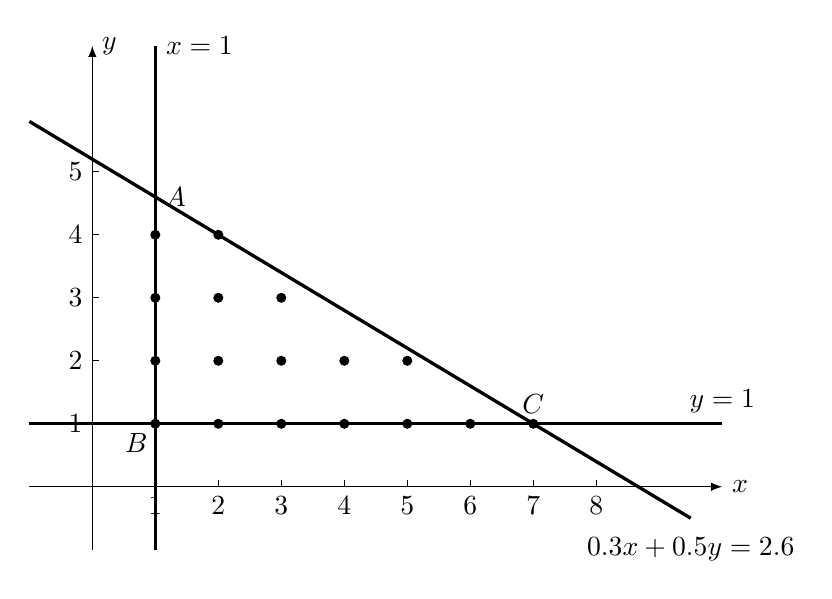
\begin{tikzpicture}[>=latex, scale=.8]
    \draw[->] (-1,0) --(10,0)node[right]{$x$};
    \draw[->] (0,-1)--(0,7)node[right]{$y$};
    \foreach \x in {1,2,...,8}
    {
        \draw (\x,0)node[below]{$\x$}--(\x,.1);
    }
\foreach \y in {1,2,...,5}
{
    \draw (0,\y)node[left]{$\y$}--(.1,\y);
}
\draw [domain=-1:9.5, samples=10, very thick] plot(\x, {5.2-0.6*\x});
\draw[very thick](-1,1)--(10,1)node[above]{$y=1$};
\draw[very thick](1,-1)--(1,7)node[right]{$x=1$};
\node at (9.5,-1){$0.3x+0.5y=2.6$};
\node at (1-.3,1-.3){$B$};
\node at (1,4.6)[right]{$A$};
\node at (7,1)[above]{$C$};

\foreach \x in {1,2,...,7}
{
    \draw (\x,1) [fill=black] circle(2pt);
}
\foreach \x in {1,2,...,5}
{
    \draw (\x,2)[fill=black] circle (2pt);
}
\foreach \x in {1,2,...,3}
{
    \draw (\x,3)[fill=black] circle (2pt);
}
\foreach \x in {1,2}
{
    \draw (\x,4) [fill=black] circle(2pt);
}

\end{tikzpicture}
    \caption{}
\end{figure}
\end{solution}

\begin{example}
 某停车场共占地36个单位,每一小汽车空位占地
2个单位,而每一大汽车空位占地3个单位,并且要使小汽
车停放辆数至少是大汽车停放辆数的两倍,问:
\begin{enumerate}
    \item 这个停车场最多可以停放多少辆汽车?
    \item 在满足上述条件下,尽可能多地停放大汽车,那么这
个停车场最多放大、小汽车各几辆?
\end{enumerate}
\end{example}


\begin{solution}
设停车场停放小汽车$s$辆,大汽车$\ell$辆.依题意$s$和$\ell$必
须满足不等式组: 
\[\begin{cases}
2s+3\ell\le 36\\
s\ge 2\ell    
\end{cases}\]
其中:$s,\ell\ge 0$,且$s,\ell$是整数.作不等式组图象,它的解集是图4.34的$\triangle OAB$围成的凸区域
(包括周界)中坐标是整数的点,由图可以看出在$A(18,0)$
点,停车场停放车辆最多,共放小汽车18辆,我们可以这样
来说明:

直线$2s+3\ell =36$,即:$s=18-\frac{3}{2}\ell$
的斜率是$-\frac{3}{2}$,因此
\[\frac{\Delta s}{\Delta \ell}=-\frac{3}{2}\]
这表示在停车场停满车辆的情形下,每次增停大汽车2辆,
小汽车就要减停3辆.于是停车场的停车总数$s+\ell=\left(18-\frac{3}{2}\ell\right)+\ell=18-\frac{1}{2}\ell$
将因$\ell$的增加而减小,故当$\ell=0$时,
$s+\ell$有最大值18.

\begin{figure}[htp]
    \centering
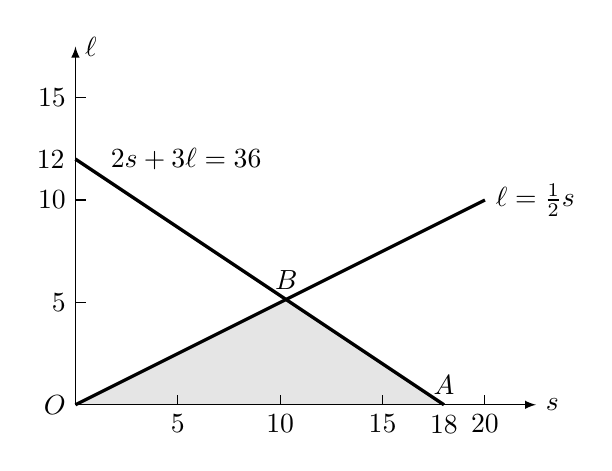
\begin{tikzpicture}[>=latex, scale=1.3]
\fill[gray!20] (0,0)--(2.06,1.03)--(3.6,0)--(0,0);

    \draw[->] (0,0) --(4.5,0)node[right]{$s$};
    \draw[->] (0,0)node[left]{$O$}--(0,3.5)node[right]{$\ell$};
\foreach \x in {5,10,15}
{
    \draw(\x/5,0)node[below]{$\x$}--(\x/5,.1);
    \draw(0,\x/5)node[left]{$\x$}--(.1,\x/5);
}
\draw(4,0)node[below]{20}--(4,.1);
\node at (0.25,2.4)[right]{$2s+3\ell=36$};
\draw[very thick](0,2.4)node[left]{12}--(3.6,0)node[below]{18};
\node at (3.6,0)[above]{$A$};
\draw[very thick] (0,0)--(4,2)node[right]{$\ell=\frac{1}{2}s$};
\node at (2.06,1.03)[above]{$B$};
\end{tikzpicture}
    \caption{}
\end{figure}



再从图看出$B$点最高,$B$点的坐标应满足方程组:
\[\begin{cases}
    2s+3\ell=36\\
s=2\ell
\end{cases}\]
解得:$\ell=5\frac{1}{7},\quad s=10\frac{2}{7}$.

在$\triangle OAB$区域内靠近$B\left(10\frac{2}{7},\; 5\frac{1}{7}\right)$点的整数值坐标的点是$(10,5)$.此点坐标符合所列不等式组,因此大汽车最多可
停放5辆,此时小汽车最多可以停放10辆.
\end{solution}
   
\section*{习题4.5}

\addcontentsline{toc}{subsection}{习题4.5}

\begin{enumerate}
    \item 画出下列不等式的图象:
\begin{multicols}{2}
    \begin{enumerate}
        \item $2x+3y\ge 6$
        \item $3x-4y\le 2$
        \item $5x-2y\ge 0$
        \item $4x+3y\le 0$
    \end{enumerate}
\end{multicols}

 \item 画出下列不等式组的图象:
 \begin{multicols}{2}
    \begin{enumerate}
        \item $\begin{cases}
            y-2x>0\\x-y-2<0
        \end{cases}$
        \item $\begin{cases}
            x+1\ge 0\\y+1\ge 0\\x+y\le 1\\ x-y\le 1
        \end{cases}$
        \item $\begin{cases}
            y-1\le 0\\2x+3y\ge 0
        \end{cases}$
        
        \item $\begin{cases}
            x-y+2\ge 0\\x-y-2\le 0\\x+y+2\le 0\\x+y-2\ge 0
        \end{cases}$
    \end{enumerate}
\end{multicols}

\item 当$(x,y)$同时满足下面不等式组时,求$x$的最大值与$y$的
    最大值,
    \[\begin{cases}
     x-y+4\ge 0\\
2x+y-4\le 0\\
x+2y+1\ge 0       
    \end{cases}\]

\item 
30个人要分乘5座与6座的出租汽车出游,车库6座车
至多只有两辆,5座车数量很多,车上有空座也无妨:
\begin{enumerate}
    \item 画出图象表示派车方案;
    \item 哪些派车办法使用车
的数目最少?在这些办法中分别有几个空座?
\end{enumerate}

\item 某小工厂每生产一件产品A获利4元,每生产一件产品
B获利5元,该厂每周至多能生产A35件,B20件,要求
每周至少获利200元,应该怎样安排生产计划?
\begin{enumerate}
    \item 写出必须满足的关系式,说明你所用字母的意义;
    \item 画出解的集合的图象;
    \item 找出使工厂盈利超过200元而生产B尽量少的各种
办法.
\end{enumerate}
\end{enumerate}

\subsection{再谈函数及其图象}
画函数图象要注意函数的定义域,如

\begin{example}
    画出下列函数的图象:
    \begin{enumerate}
        \item $y=2x,\qquad (x\in\mathbb{R})$;
        \item $y=2x,\qquad (0\le x\le 5)$;
        \item $y=2x$,\qquad ($x$是整数).
    \end{enumerate}
\end{example}


\begin{solution}
1的图象是图4.35(a)的直线$AB$; 2的图象是
图4.35(b)的线段$CD$; 3的图象是图4.35(c)的一些离散
的点.

\begin{figure}[htp]
    \centering
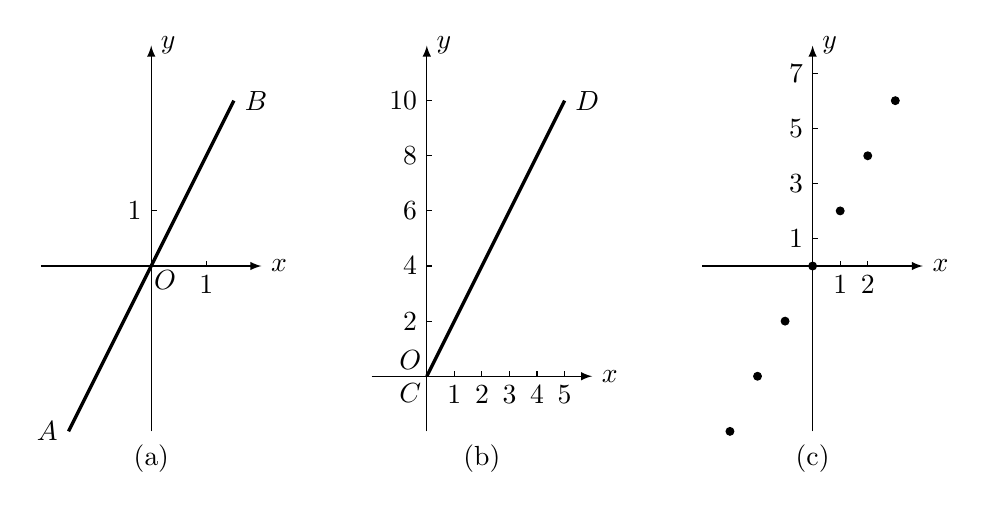
\begin{tikzpicture}[>=latex, scale=.7]
\begin{scope}
    \draw[->] (-2,0) --(2,0)node[right]{$x$};
    \draw[->] (0,-3)--(0,4)node[right]{$y$};
    \draw[very thick](-1.5,-3)node[left]{$A$}--(1.5,3)node[right]{$B$};
    \draw (0,1)node[left]{1}--(.1,1);
    \draw (1,0)node[below]{1}--(1,.1);
    \node at (.25,-.25){$O$};

    \node at (0,-3.5){(a)};
\end{scope}
\begin{scope}[xshift=5cm, yshift=-2cm]
    \draw[->] (-1,0) --(3,0)node[right]{$x$};
    \draw[->] (0,-1)--(0,6)node[right]{$y$};
    \draw[very thick](0,0)--(2.5,5)node[right]{$D$};
\foreach \x in {1,2,...,5}
{
    \draw(\x/2,0)node[below]{$\x$}--(\x/2,.1);
}
\foreach \x in {2,4,...,10}
{
    \draw (0,\x/2)node[left]{$\x$}--(.1,\x/2);
}
\node at  (-.3,-.3){$C$};
\node at  (-.3,.3){$O$};
\node at (1,-1.5){(b)};
\end{scope}
\begin{scope}[xshift=12cm]
    \draw[->] (-2,0) --(2,0)node[right]{$x$};
    \draw[->] (0,-3)--(0,4)node[right]{$y$};
    \foreach \x in {1,2}
    {
        \draw(\x/2,0)node[below]{$\x$}--(\x/2,.1);
    }
    \foreach \x in {1,3,5,7}
    {
        \draw (0,\x/2)node[left]{$\x$}--(.1,\x/2);
    }
\foreach \x in {-3,-2,...,3}
{
    \draw (\x/2,\x) [fill=black] circle(2pt);
}
\node at (0,-3.5){(c)};
\end{scope}

\end{tikzpicture}
    \caption{}
\end{figure}
\end{solution}

从这里我们再次体会到,当谈论函数时是离不开定义域
的,因为若函数表达式一样,而其定义域不同,则它们的图象
会差之干里,故例中1、2、3三个函数不能认为是相
同的函数.

有时用公式表示的函数,在它的定义域的不同部分可以
用不同的公式表示,即可用若干公式表示变量间的关系,请
看下例:


\begin{example}
 火车在9小时内从A行驶到B, 在最初三小时内,
它的行驶速度为50公里/小时,接下来它停止了两小时,在最
后的四小时内,它以速度60公里/小时行驶到达B. 试表示行
车路程和时间的关系.
\end{example}


\begin{solution}
以$x$表示时间,单位为小时;以$y$表示走过的路程,
单位为公里,我们就得到下面的函数式$y=f(x)$:
\[y=f(x)=\begin{cases}
   50x& 0\le x\le 3\\
150 &3\le x\le 5\\
150+60(x-5)& 5\le x\le 9 
\end{cases}\]
显见,对于定义域$[0,9]$内每一个$x$值,$y$就有唯一确定的值
和它对应,因而$f(x)$是个定义在$[0,9]$上的函数,但这个函
数是用几个不同的式子给出来的,这个函数的图象画在图
4.36中.

\begin{figure}[htp]
    \centering
\begin{tikzpicture}[>=latex,scale=.7]
    \draw[->] (-1,0) --(9,0)node[right]{$x$(小时)};
    \draw[->] (0,-1)--(0,9)node[right]{$y$(公里)};
\foreach \x/\y in {1/50,2/100,3/150,4/200,5/250,6/300,7/350,8/400}
{
    \draw (\x,0)node[below]{$\x$}--(\x,.1);
    \draw (0,\x)node[left]{$\y$}--(.1,\x);
}
    \node at (-.5,-.5){$O$};
\draw[very thick](0,0)--node[rotate=45, above]{$y=50x$}(3,3)--node[above]{$y=50$}(5,3)--node[rotate=52, above]{$y=150+60(x-5)$}(9,7.8);

\end{tikzpicture}
    \caption{}
\end{figure}
    
\end{solution}


\begin{example}
    画出函数$y=|x|$的图象.
\end{example}




\begin{solution}    
这个函数的定义域是一切实数,按照绝对值的定义
    我们有:
\[y=|x|=\begin{cases}
    x&x\ge 0\\
    -x&x<0
\end{cases}\]
图象是折线(图4.37).
\begin{figure}[htp]
    \centering
\begin{tikzpicture}[>=latex]
    \draw[->] (-3,0) --(3,0)node[right]{$x$};
    \draw[->] (0,0)--(0,3)node[right]{$y$};
    \draw (1,0)node[below]{$1$}--(1,.1);
    \draw (0,1)node[left]{$1$}--(.1,1);
    \node at (0,0)[below]{$O$};
\draw[very thick] (-2,2)--(0,0)--(2,2);
\end{tikzpicture}
    \caption{}
\end{figure}
\end{solution}    

\begin{example}
    已知$f(x)=|x+1|+\sqrt{(x-2)^2}$
\begin{enumerate}
    \item 求函数的定义域;
    \item 当$-1\le x<2$时,化简函数的解析式;
    \item 作出函数的图象,并说明函数的值域是什么?
\end{enumerate}
\end{example}    

\begin{solution}
\begin{enumerate}
    \item 对于$|x+1|$, $x$可取一切实数;对于$\sqrt{(x-2)^2}$,
    $x$必须满足$(x-2)\ge 0$, 这个不等式对于一切实数都成立,
    所以函数的定义域是一切实数.
\item $\sqrt{(x-2)^2}=|x-2|$, $f(x)=|x+1|+|x-2|$,
    要脱掉绝对值符号需分段讨论.我们知道$x=-1$时,
    $|x+1|=0$; $x=2$时,$|x-2|=0$, 故$-1,2$把数轴
    分为三段:$(-\infty,-1)$, $[-1,2)$, $[2,+\infty)$.
\begin{itemize}
    \item 当$x\in (-\infty,-1)$时,
    $$f(x)=|x+1|+|x-2|=-(x+1)-(x-2)=-2x+1$$
    \item 当$x\in[-1,2)$时,$f(x)=(x+1)-(x-2)=3$
  \item   当$x\in [2,+\infty)$时,$f(x)=(x+1)+(x-2)=2x-1$
\end{itemize}
即:\[f(x)=\begin{cases}
   -2x+1  & x<-1\\
   3& -1\le x<2\\
   2x-1 & x\ge 2 
\end{cases}\]
\item 画出的图象是图4.38.
由观察图象知:
\begin{itemize}
    \item 当$x<-1$时,$f(x)=-2x+1>3$;
    \item 当$-1\le x<2$时,$f(x)=3$;
    \item 当$x\ge 2$时,$f(x)=2x-1\ge 3$
\end{itemize}
所以函数的值域是$f(x)\ge 3$的一切实数.
\end{enumerate}

\begin{figure}[htp]
    \centering
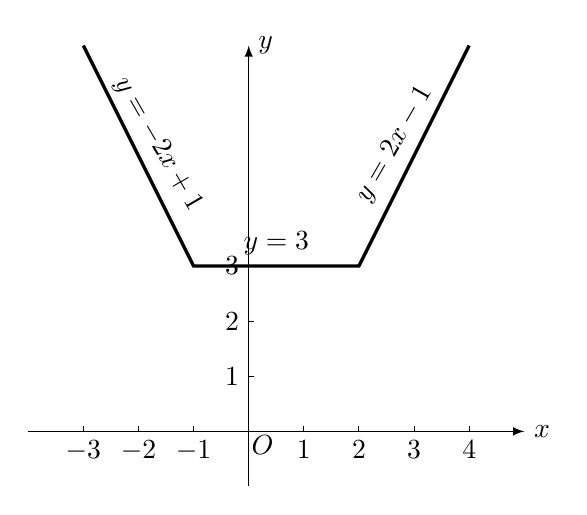
\begin{tikzpicture}[>=latex, scale=.7]
    \draw[->] (-4,0) --(5,0)node[right]{$x$};
    \draw[->] (0,-1)--(0,7)node[right]{$y$};
\foreach \x in {-3,-2,-1,1,2,3,4}
{
    \draw (\x,0)node[below]{$\x$}--(\x,.1);
}
\foreach \y in {1,2,3}
{
    \draw (0,\y)node[left]{$\y$}--(.1,\y);
}

\draw [very thick](-3,7)--node[rotate=-60, above]{$y=-2x+1$}(-1,3)--node[above]{$y=3$}(2,3)--node[rotate=60, above]{$y=2x-1$}(4,7);


    \node at (0.25,-0.25){$O$};

\end{tikzpicture}
    \caption{}
\end{figure}


\end{solution}

下面我们再来看一类函数作为本章的结束.

\begin{example}
邮局规定,寄往外埠普通信件重量不超过20克者
邮资8分,重量超过20克但不超过40克者,邮资1角6分,
重量超过40克但不超过60克者,邮资2角4分,依此每增加
20克邮资增加8分,因此邮资是重量$x$的函数,函数的图象
为图4.39.
\begin{figure}[htp]
    \centering
\begin{tikzpicture}[>=latex]
    \draw[->] (-1,0) --(6,0)node[right]{$x$(克)};
    \draw[->] (0,-1)--(0,6)node[right]{$y$(分)};
    \foreach \x in {20,40,...,100}
    {
        \draw (\x/20,0)node[below]{$\x$}--(\x/20,.1);
    }
    \foreach \y in {8,16,...,40}
    {
        \draw (0,\y/8)node[left]{$\y$}--(.1,\y/8);
    }
    \node at (-0.25,-0.25){$O$};
\draw[very thick]  (0,1)--(1,1);
\draw[very thick]  (1,2)--(2,2);
\draw[very thick]  (2,3)--(3,3);
\draw[very thick]  (3,4)--(4,4);
\draw[very thick]  (4,5)--(5,5);
\foreach \x in {1,2,3,4}
{
    \draw (\x, \x+1) [fill=white] circle (1.5pt);
}
\end{tikzpicture}
    \caption{}
\end{figure}

这种类型的函数称为阶梯函数,它的特点是:自变量$x$
的变化范围分成若干区间,在每个区间中,因变量$y$的值是
不变的,但对应不同区间,$y$值是可以不同的,在每个区间
的端点处,因变量$y$的值有一个跳跃,也就是说函数的图象
不是连续的,而有间断的地方.

例4.27和例4.30中的函数从总体看也是递增变化的,但有时
不增也不减处在平稳状态,这样的函数称为不减的.

    
\end{example}

\begin{blk}{定义}
    如果对于开区间$(a,b)$(或闭间$[a,b]$)的任意两个
  自变量的值$x_1$和$x_2$:
  \begin{itemize}
      \item 当$x_1<x_2$时,可以推出$f(x_1)\le f(x_2)$, 那么
  函数$f(x)$称为在开区间$(a,b)$(或闭区间$[a,b]$上)\textbf{不减}.
\item  当$x_1<x_2$时,可以推出$f(x_1)\ge f(x_2)$, 那么函数$f(x)$称
  为在开区间(或闭区间$[a,b]$上\textbf{不增}.   
  \end{itemize}
  \end{blk}
  
  
  



\section*{习题4.6}

\addcontentsline{toc}{subsection}{习题4.6}

\begin{enumerate}
    \item 作函数图象:
   \[y=f(x)=\begin{cases}
       x& 0\le x<2\\
       2& 2\le x<4\\
       -x+6 & 4\le x<6
   \end{cases}\]
   \item 作函数图象:
    $y=-|x+1|$
    \item 作函数图象:
   \[f(x)=\begin{cases}
       2& x\le -1\\
       1-x& -1<x\le 0\\
       1+x & 0<x\le 1\\
       2& x>1
   \end{cases}\]
    \item 一列火车在$t=0$时由A地开出,速度是每小时100公里,
    行驶2小时到达B地;在那里停车1小时后,以每小时
    80公里的速度继续向前行驶3小时,表示火车在时刻$t$与
    A地的距离(单位:公里)的函数.
    \item 作出函数$y=|x-2|-2$的图象,并求出它与$x$轴所围
    成的图形的面积.
\end{enumerate}

\section*{复习题四}
\addcontentsline{toc}{section}{复习题四}

\begin{enumerate}
    \item 叙述函数的定义域与值域.
    \item 指出下列函数的定义域与值域:
\begin{multicols}{2}
\begin{enumerate}
    \item $f(x)=\sqrt{x}$
    \item $f(x)=1-|x|$
    \item $f(x)=\frac{1}{\sqrt{x^2+1}}$
    \item $f(x)=\sqrt{4x-1}$
\end{enumerate}
\end{multicols}
    
    \item 指出下列函数的定义域:
\begin{multicols}{2}
\begin{enumerate}
\item $f(x)=\frac{\sqrt{x+1}}{\sqrt{x-1}}$
\item $f(x)=\frac{\sqrt{x+4}}{x-5}$
\item $f(x)=\frac{6}{x^2-3x+2}$
\item $f(x)=\frac{\sqrt{4x+8}}{3x-2}$
\item $f(x)=\sqrt{2x-1}+1-2x+x^2$
\item $f(x)=\frac{1}{x+5}+\lg(-x)$
\end{enumerate}
\end{multicols}
    \item 作出下列函数的图象:
\begin{enumerate}
    \item $f(x)=2x,\qquad x\in\{-2,-1,0,1,2\}$
    \item $f(x)=-2x+1,\qquad x\ge 1$
    \item $f(x)=-x-2,\qquad -2<x\le 2$
    \item $f(x)=\begin{cases}
        1&x>0\\-1&x\le 0
    \end{cases}$
    \item $f(x)=\begin{cases}
        -x+6  &  x>2\\
        x^2& -2\le x\le 2\\
        x+6& x<-2
    \end{cases}$
\end{enumerate}

\item 在同一坐标系里,作出下面三个函数的图象,并说明这
三个图象的形状和位置有何关系:
\[y=7x;\qquad y=7x+3;\qquad y=7x-3\]
\item 
按照下列各组条件,确定一次函数$y=f(x)$:
\begin{multicols}{2}
\begin{enumerate}
    \item $f(0)=3,\qquad f(-1)=-1$
    \item $f(1)=2,\qquad f(-1)=1$
    \item $f(0)=-3,\qquad f\left(\frac{3}{2}\right)=0$
    \item $f(1)=1,\qquad f(0)=-2$
    \item $f(0)=0,\qquad f(5)=-7$
\end{enumerate}
\end{multicols}
\item 已知$P_1(1,1)$及$P_2(5,13)$两点在直线$y=kx+b$上,
试求出$k$和$b$, 并画出图象,点$P(3,7)$是否在这条直线上?
\item 长为12cm的弹簧,能承受的重量在0—15千克的范围内,
重量每增加1千克,弹簧被拉长0.5cm, 试写出承受的
重量$x$(千克)与弹簧长$y$(厘米)之间的函数关系式,并作
出图象.
\item 
行星绕太阳一周所需日数的平方,与行星离太阳的距离
的立方成正比例,已知地球绕太阳一周约需365日,水星
绕太阳一周约需88日,地球离太阳约$1.5\x10^8$公里,求
水星离太阳约多少公里?
\item 海上所能看到的水面距离,与眼晴离海平面的高的平
方根成反比例.如果眼晴离海平面高2米时,所能看到的
水面距离是5公里,那么眼晴离海平面高是8米时,能
看到的距离是多少公里?
\item 如果变量$y$与$x$成反比例,变量$z$与$y$也成反比例,求证
变量$z$与$x$成正比例.
\item 在同一坐标系里,对$k,b$的下列数值,作出函数
$y=k|x|+b$的图象,并说明这些图象的形状和位置有
何关系?
\begin{multicols}{2}
\begin{enumerate}
    \item $k=3,\qquad b=5$
    \item $k=-3,\qquad b=5$
    \item $k=4,\qquad b=0$
    \item $k=-4,\qquad b=0$
    \item $k=\frac{1}{2},\qquad b=3$
    \item $k=-\frac{1}{2},\qquad b=4$
\end{enumerate}
\end{multicols}

\end{enumerate}

